\chapter{Hadronic Resonance Identification}
\label{sec:jets}

In this chapter, we describe the reconstruction and identification of heavy ($\gtrsim 100$ GeV) resonances that decay to two or more quarks.
Within the Standard Model, the only such resonances are the massive vector bosons ($W,Z\rightarrow q\bar{q}'$), the Higgs boson (typically $H\rightarrow b\bar{b}$), and the top quark ($t\rightarrow bW(\rightarrow q\bar{q}')$).
These quarks hadronize into jets (described in Chapter~\ref{sec:theory}), which are typically reconstructed at the LHC using the anti-$k_\mathrm{T}$ algorithm (described in Chapter~\ref{sec:cms}).
The focus of this chapter is on the cases in which the resonance is boosted and the decay products merge, such that they cannot be identified as 2 or 3 distinct jets.
In preparation for Chapter~\ref{sec:mt}, we will take the top quark as a concrete example.
The studies presented here can (and in some cases have been) applied to other heavy resonances, both within and beyond the Standard Model.

\section{Reconstruction}
\label{sec:jets:reco}

The approximate angular separation between the quarks from a heavy resonance decay is\needcite:
\begin{equation}
    \Delta R \sim \frac{2M}{\pt}
\end{equation}
where $M$ is the resonance mass and $\pt$ is the resonance transverse momentum.
Setting $M=m_t$ and $\Delta R=1.2$ (i.e. the radius at which three $R=0.4$ jets start to overlap), we extract a ``merging scale'' of $300$ GeV.  
This is be verified by checking the distribution of the ``decay radius'' in top quark simulation.
Here, we define decay radius as: 
\begin{equation}
    \max\Delta R_{qq} \equiv \displaystyle\max_{0\leq i < j \leq 2} \{\Delta R(q_i,q_j)\} \text{, where } t\rightarrow q_0q_1q_2
\end{equation}
Using a broad spectrum of generated top quark $\pt$, Figure~\ref{fig:jets:dr} shows the dependence of the decay radius on the top quark $\pt$, where we restrict the resonance to satisfy $|\eta|<2.5$.
If we are interested in top quarks with $\pt>250$ GeV (motivated by the trigger selection (Section~\ref{sec:mt:sel})), then over half of top quarks will be fully contained within a jet of radius $1.5$.
That is, at $\pt\approx 250$ GeV, it is equally likely that a top quark's decay products will fall within a single large-radius jet or that they will be resolvable as three separate jets. 
However, past this threshold momentum, the large-radius jet becomes the preferred reconstruction option.
This motivates the use of $R=1.5$ jets to reconstruct hadronic top quarks with $\pt>250$ GeV. 

\begin{figure}[]
    \begin{center}
        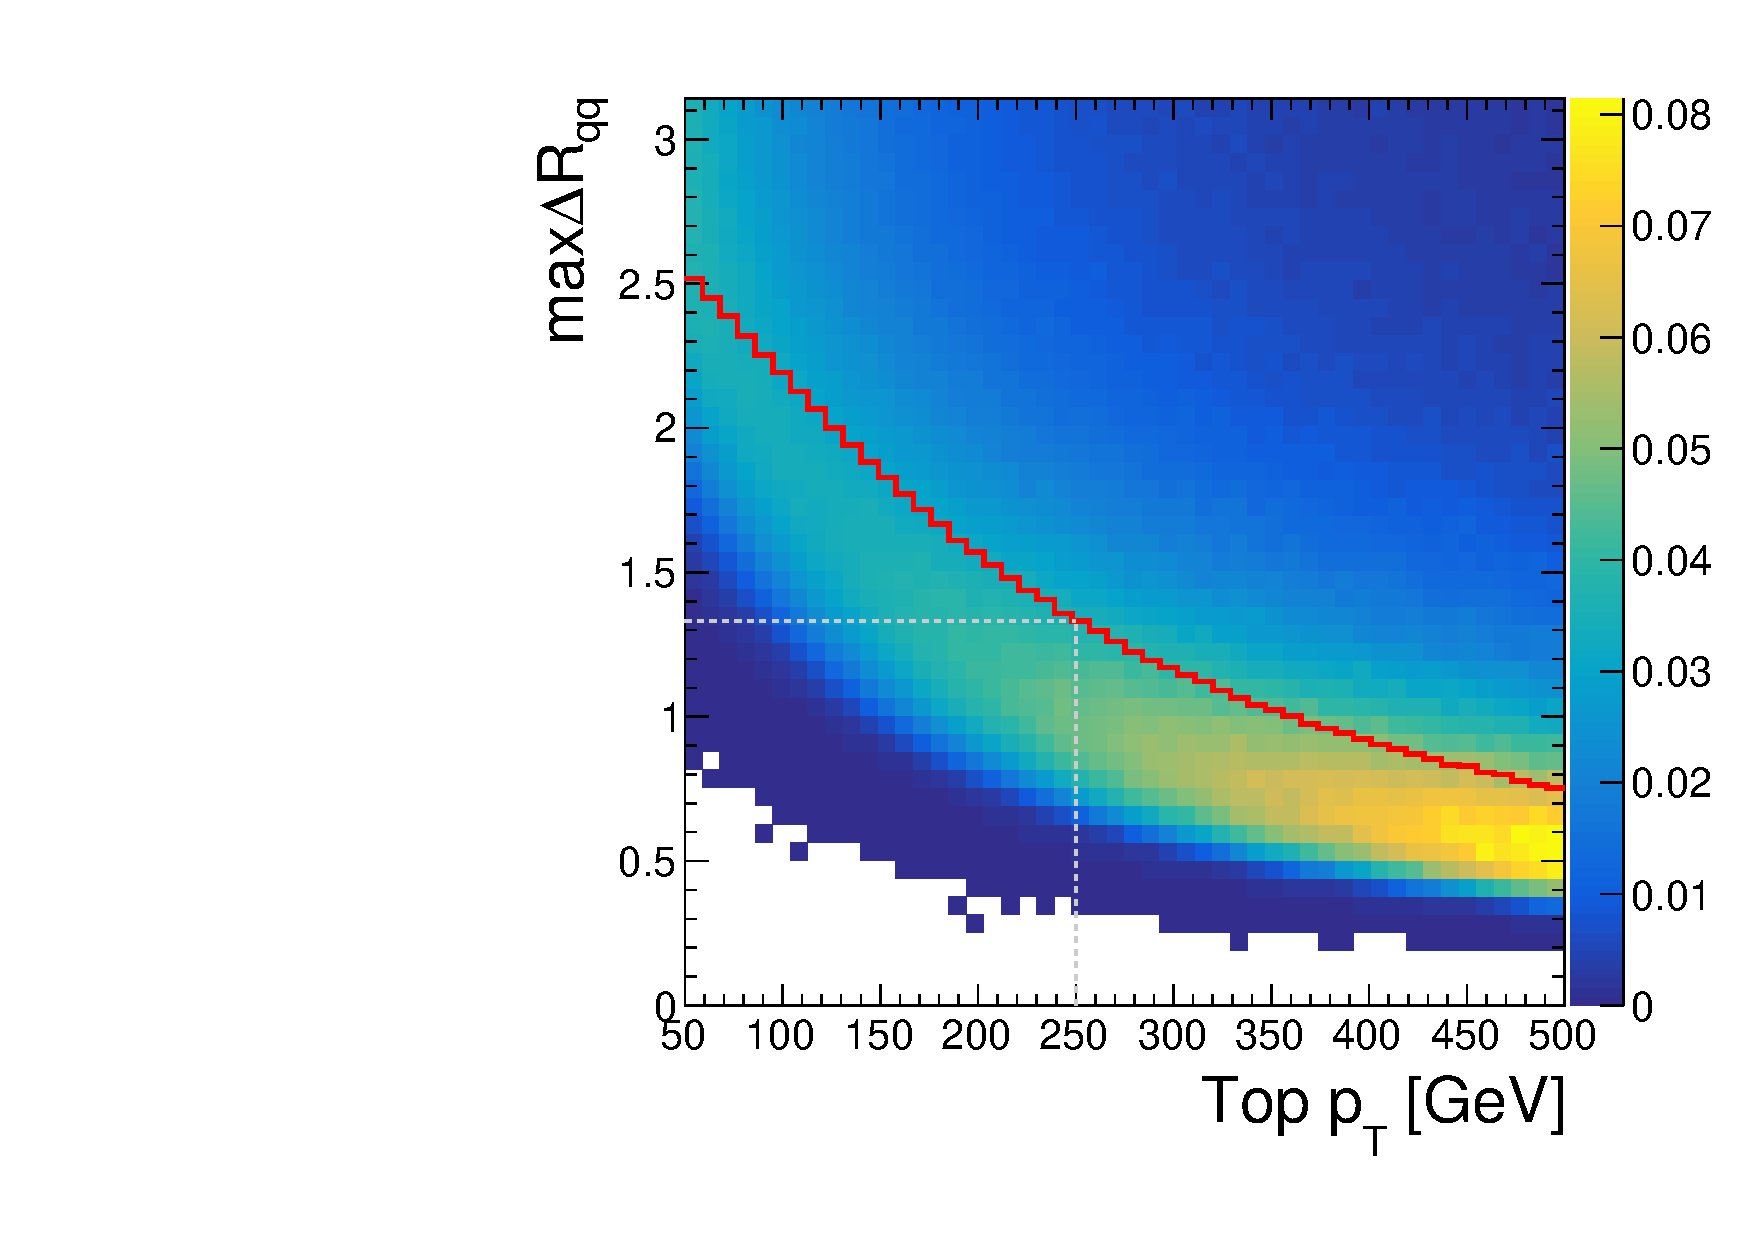
\includegraphics[width=0.5\textwidth]{figures/toptagging/gen/ptdr.pdf}
        \caption{Distribution of top quark momenta versus decay radii in a simulated top quark pair sample.
                 The events are weighted such that the inclusive momentum distribution is uniform. 
                 The $z$-axis units are arbitrary, but proportional to the distribution of jets. 
                 The solid red line marks the 50\% quantile of jets at each value of $\pt$. }
        \label{fig:jets:dr}
    \end{center}
\end{figure}

There are two tunable parameters in jet reconstruction.
We have specified the jet radius, but we must also choose the jet algorithm.
The anti-$k_\mathrm{T}$ algorithm tends to pick circular jets, whereas the Cambridge-Aachen (CA) algorithm allows for more geometric shapes (Figure~\ref{fig:jets:algos}).
As the top jets we seek to reconstruct are the sum of three light quark jets, we do not necessarily expect the $R=1.5$ jet to be circular.
Figure~\ref{fig:jets:caak} compares the jet mass distribution for top and light quark/gluon (LQG) jets, where the jets are clustered using both algorithms.
CA produces a top jet mass distribution with a narrower peak that sits closer to $m_t$ than anti-\kt. 
Because of this, and the general improvement in $S/B$ near the top mass peak, we choose the CA algorithm.
Hereafter, we will refer to Cambridge-Aachen $R=1.5$ jets as CA15 jets. 

\begin{figure}[]
    \begin{center}
        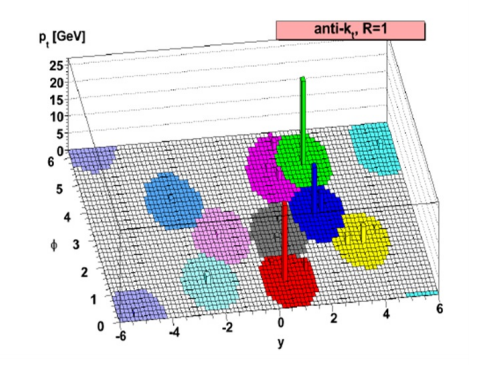
\includegraphics[width=0.35\textwidth]{figures/toptagging/gen/ak.png}
        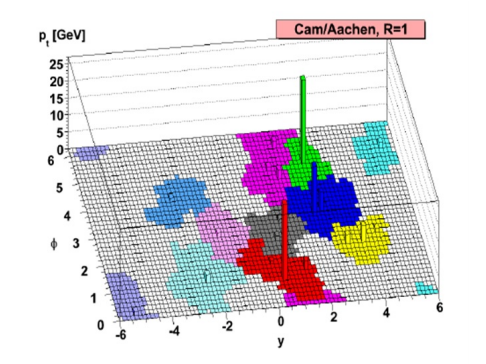
\includegraphics[width=0.35\textwidth]{figures/toptagging/gen/ca.png}
        \caption{Jets clustered using the anti-$k_\mathrm{T}$ (left) and CA (right) algorithms.
                 Shown is the $y$-$\phi$ plane of a hypothetical calorimeter, unrolled onto a flat surface.
                 The height of each cell represents the \pt~of the particle. 
                 The anti-\kt~jets tend to be more circular when compared to the CA jets.
                 Figures are adapted from~\needcite.}
        \label{fig:jets:algos}
    \end{center}
\end{figure}

\begin{figure}[]
    \begin{center}
        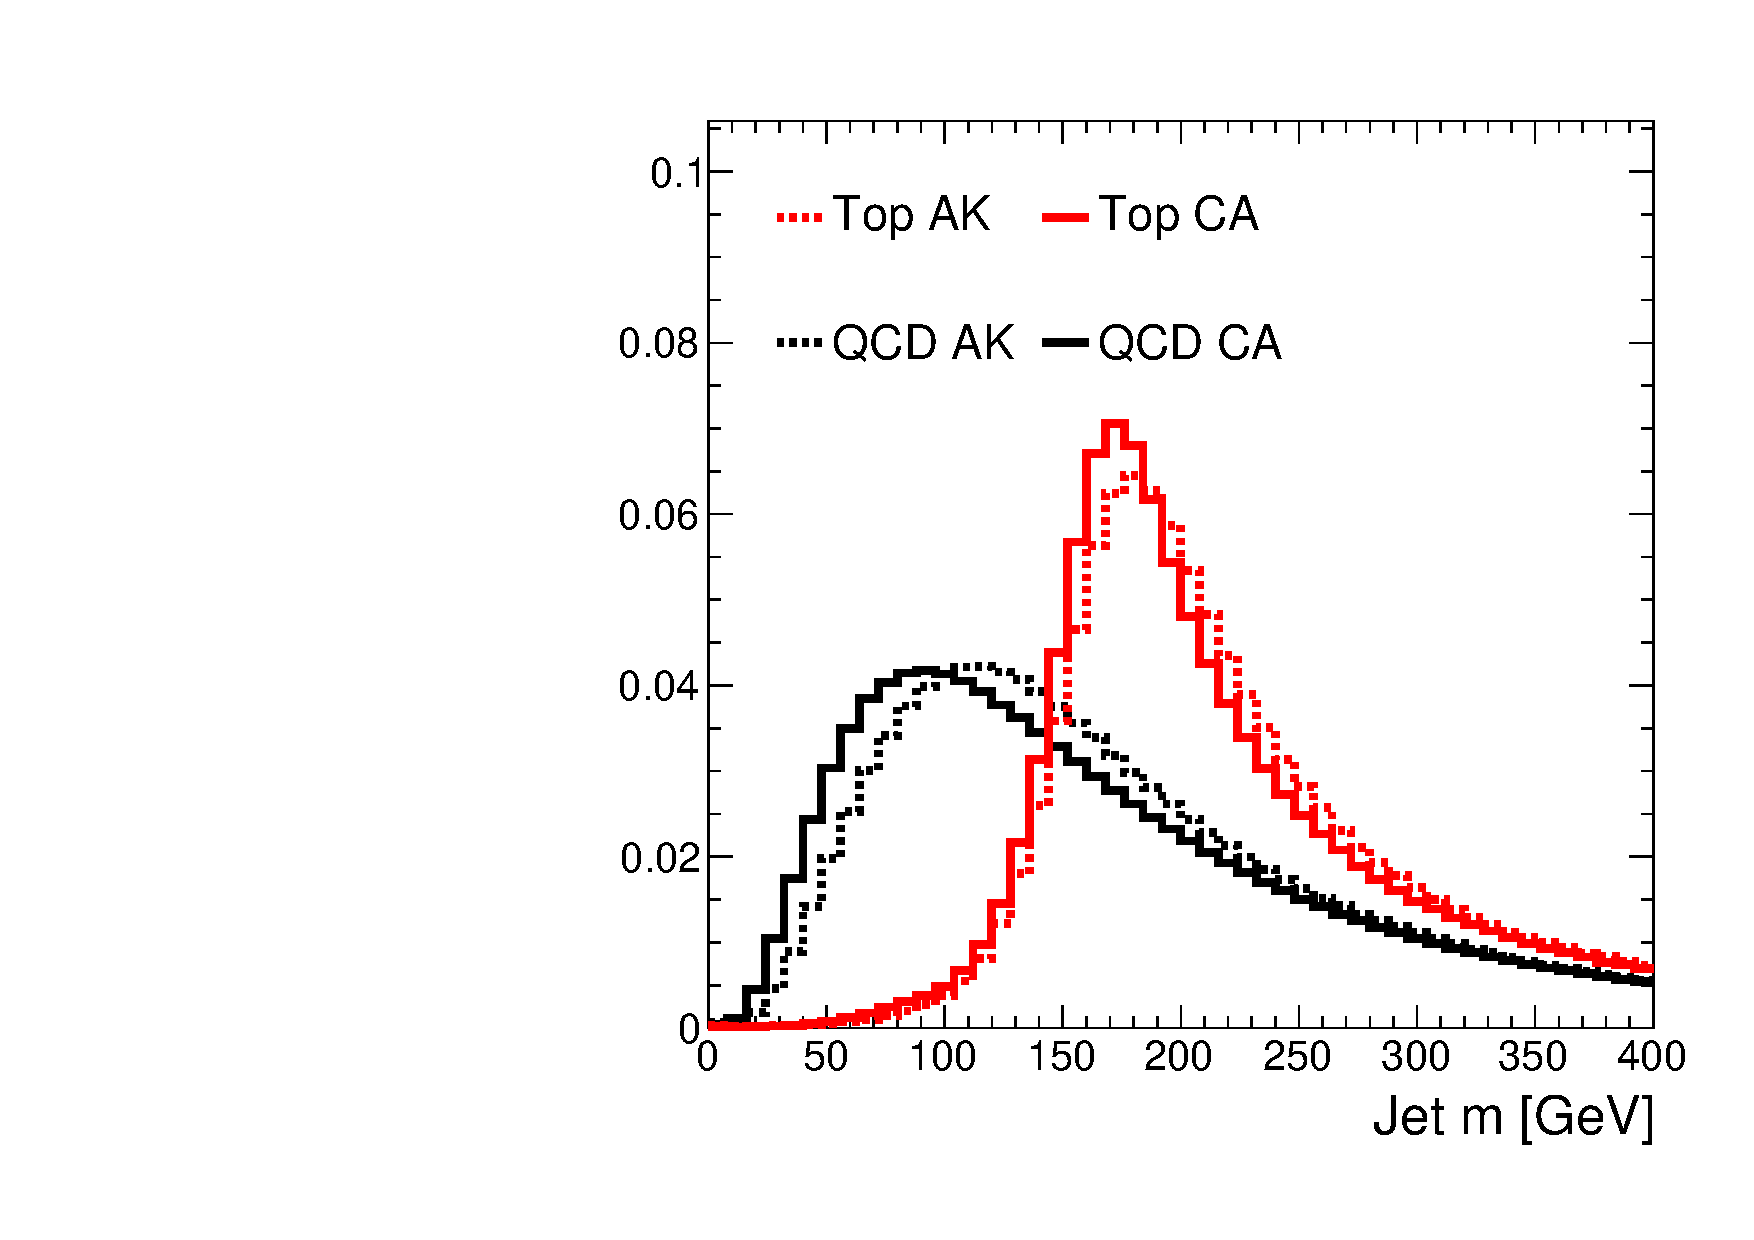
\includegraphics[width=0.5\textwidth]{figures/toptagging/gen/clf_M.pdf}
        \caption{Mass distribution for jets clustered using the anti-$k_\mathrm{T}$ (dashed) and CA (solid) algorithms.
                 QCD refers to jets originating in QCD multijet events, i.e. from the hadronization of light quarks or gluons.}
        \label{fig:jets:caak}
    \end{center}
\end{figure}

The distance parameter of $R=1.5$ corresponds approximately to a maximal azimuthal angle separation of $\nicefrac{\pi}{2}$, which can cover half of the detector's fiducial volume.
As the jet is so large, particles from pile-up interactions may accidentally be clustered into a jet from the primary vertex.
Fundamental quantities (like top quark momentum) are uncorrelated with the number of primary vertices (\NPV), but reconstructed quantities acquire such a dependence due to the extra radiation.
These additional particles bias the energy scale of the jet (e.g. the mass) as well as geometric observables (described in Section~\ref{sec:jets:id}).
To mitigate these effects, we scale the particles' 4-momenta by their corresponding PUPPI scores (described in Chapter~\ref{sec:cms}) prior to clustering the jet.
Jets clustered using all particles (without PUPPI filtering) have a jet mass and $\tau_{32}^\mathrm{SD}$ distributions (Figure~\ref{fig:jets:puppi}) in which both the mean and variance have an \NPV-dependence.
Adding PUPPI stabilizes the mean and ensures that the variance does not grow at large \NPV.

\begin{figure}[]
    \begin{center}
        \begin{subfigure}[t]{0.35\textwidth}
            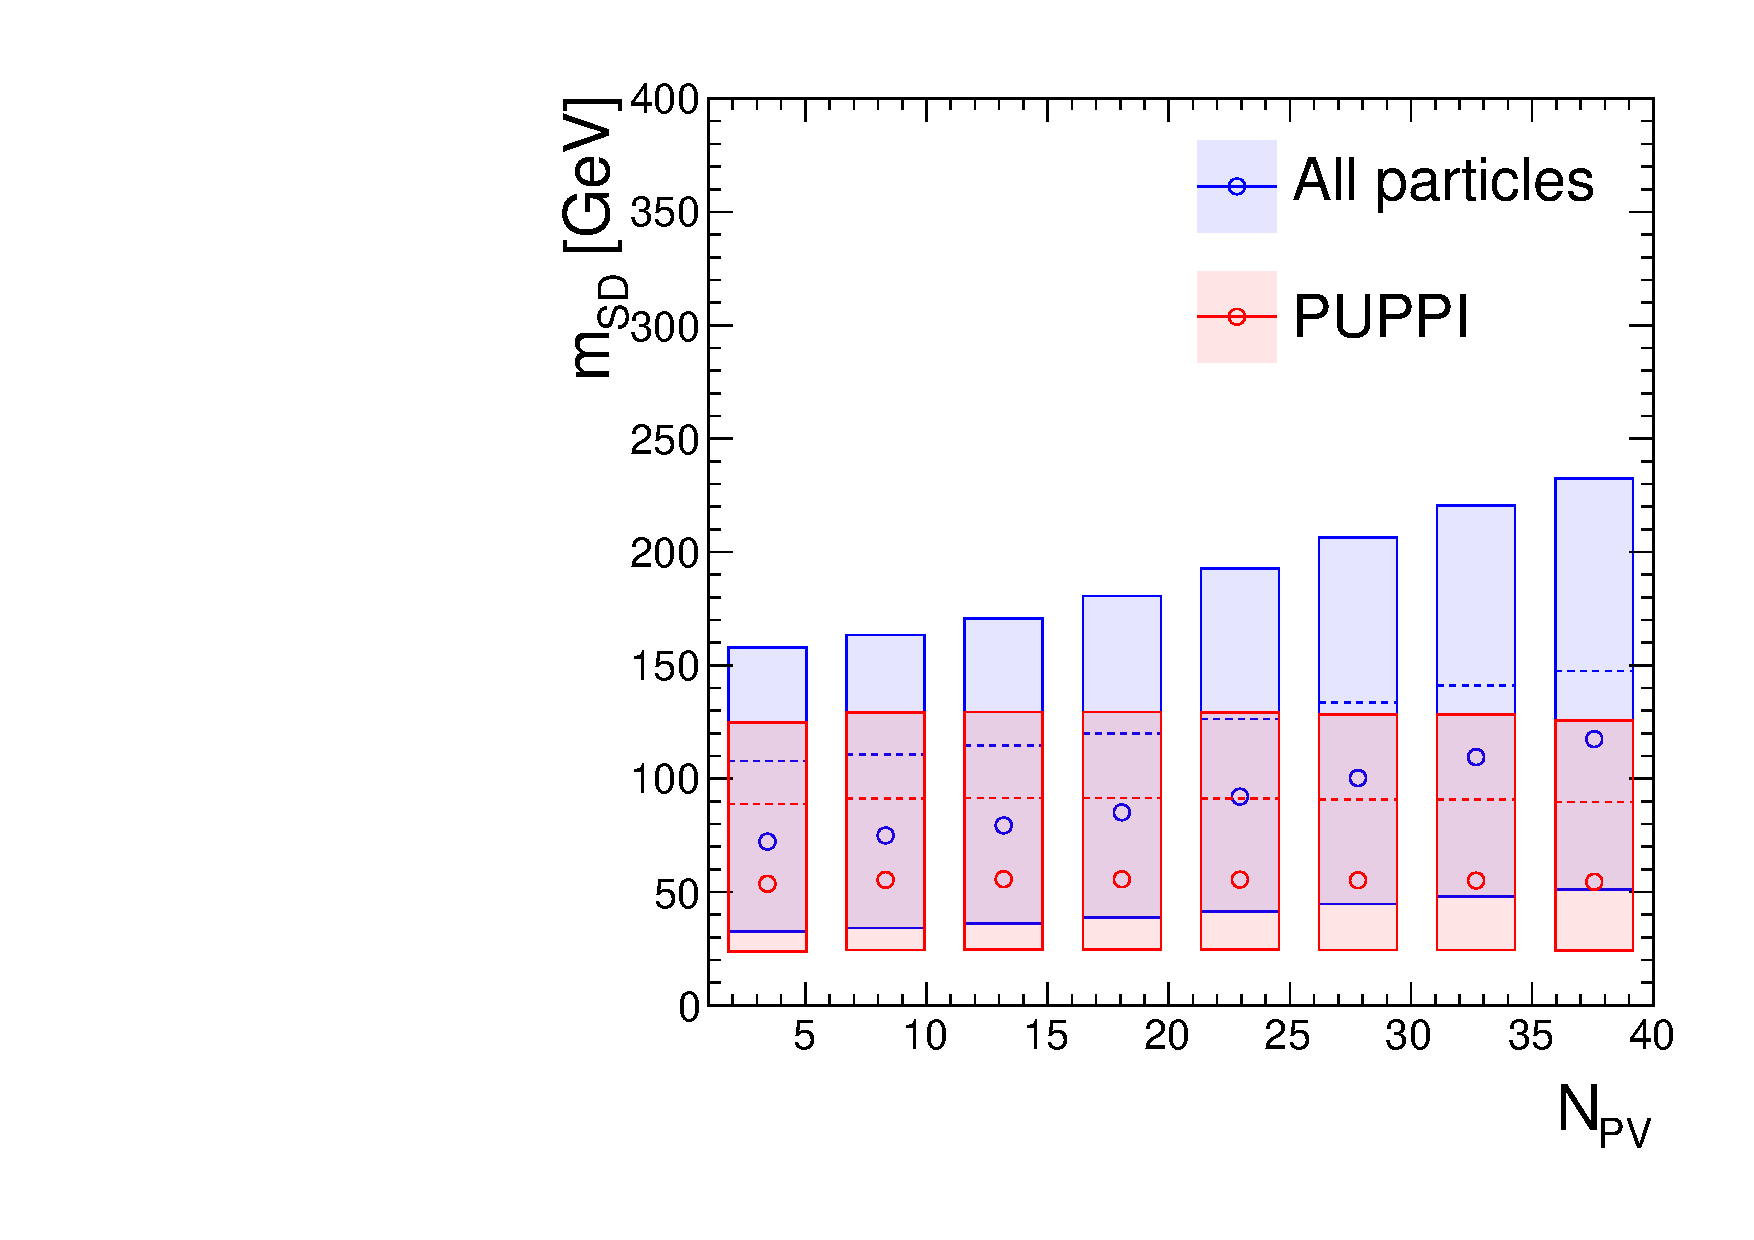
\includegraphics[width=\textwidth]{figures/toptagging/gen/npv_clf_MSD_QCD.pdf}
            \caption{Jet mass, LQG}
        \end{subfigure}
        \begin{subfigure}[t]{0.35\textwidth}
            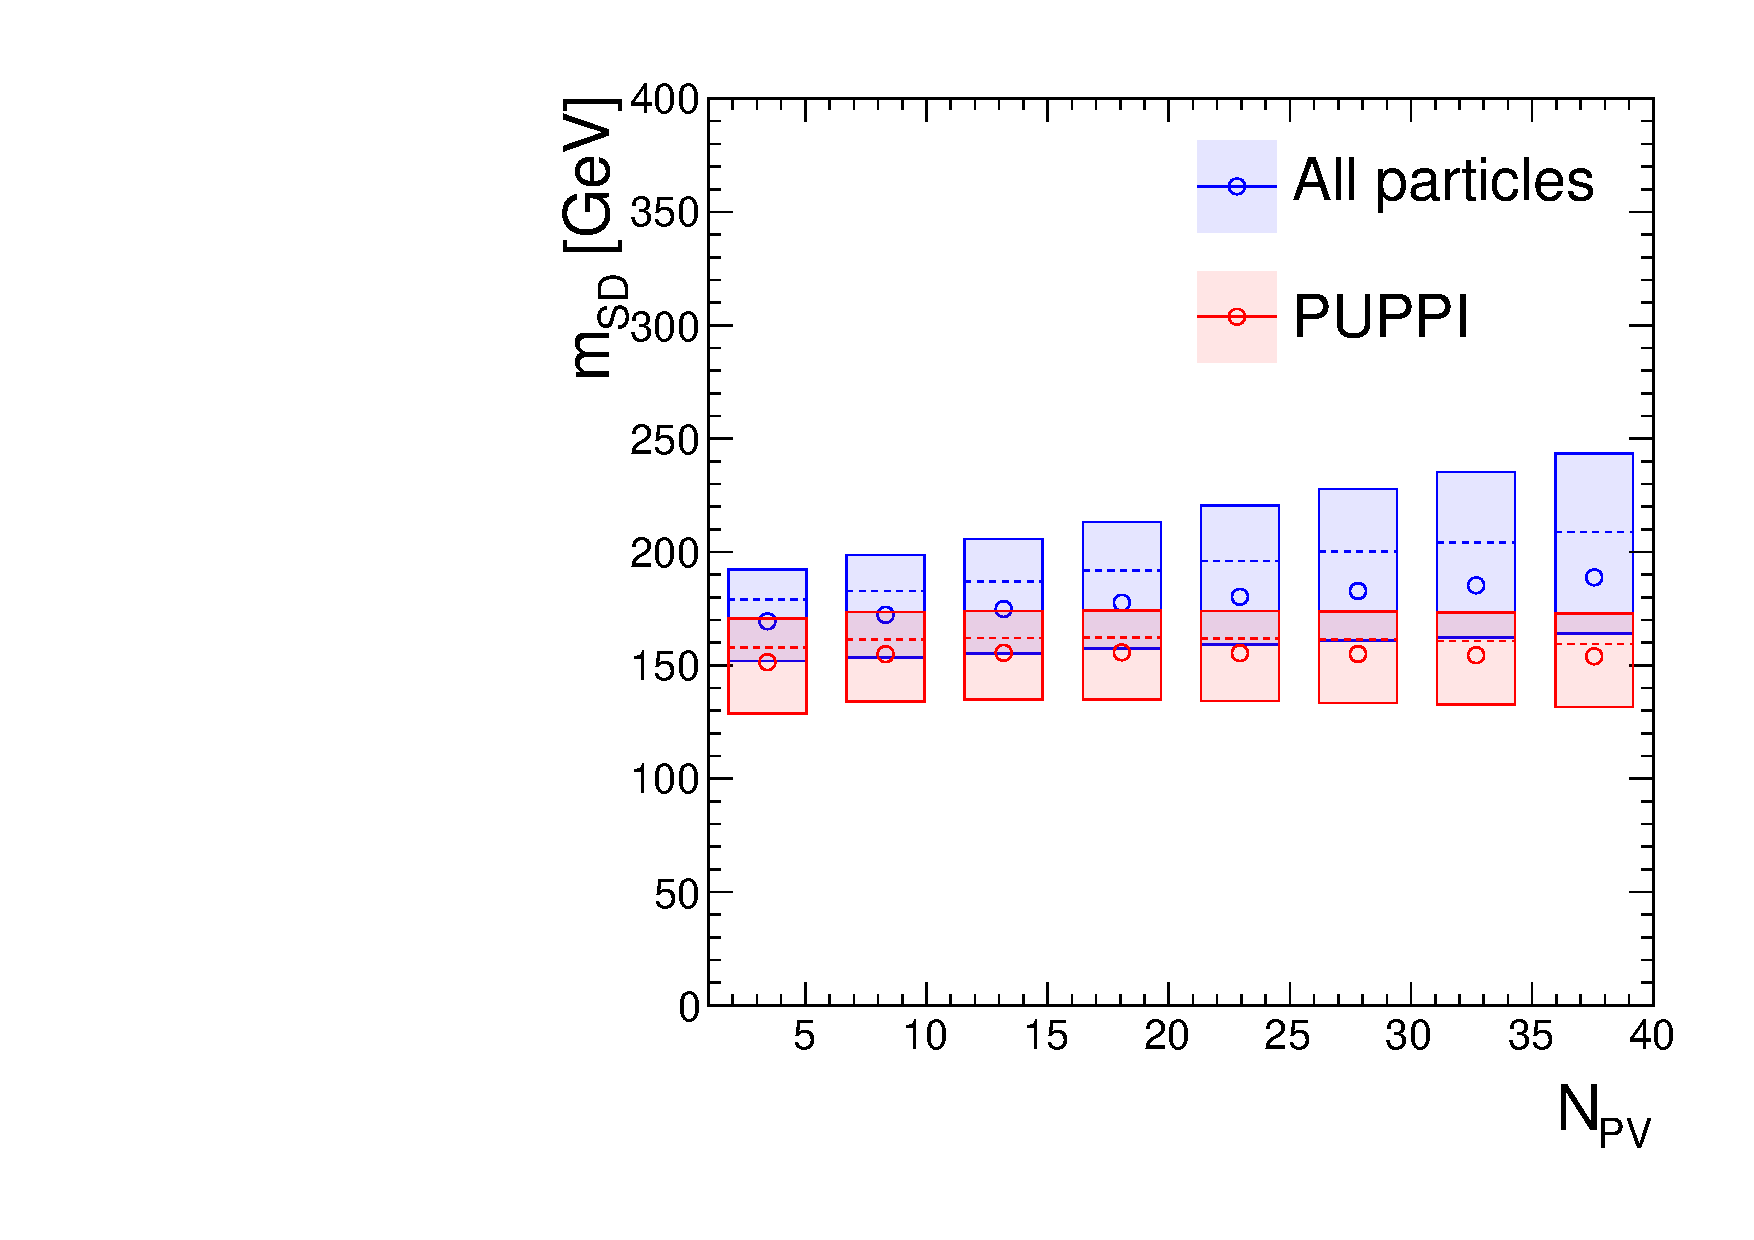
\includegraphics[width=\textwidth]{figures/toptagging/gen/npv_clf_MSD_ZpTT_lo.pdf}
            \caption{Jet mass, Top}
        \end{subfigure}
        \begin{subfigure}[t]{0.35\textwidth}
            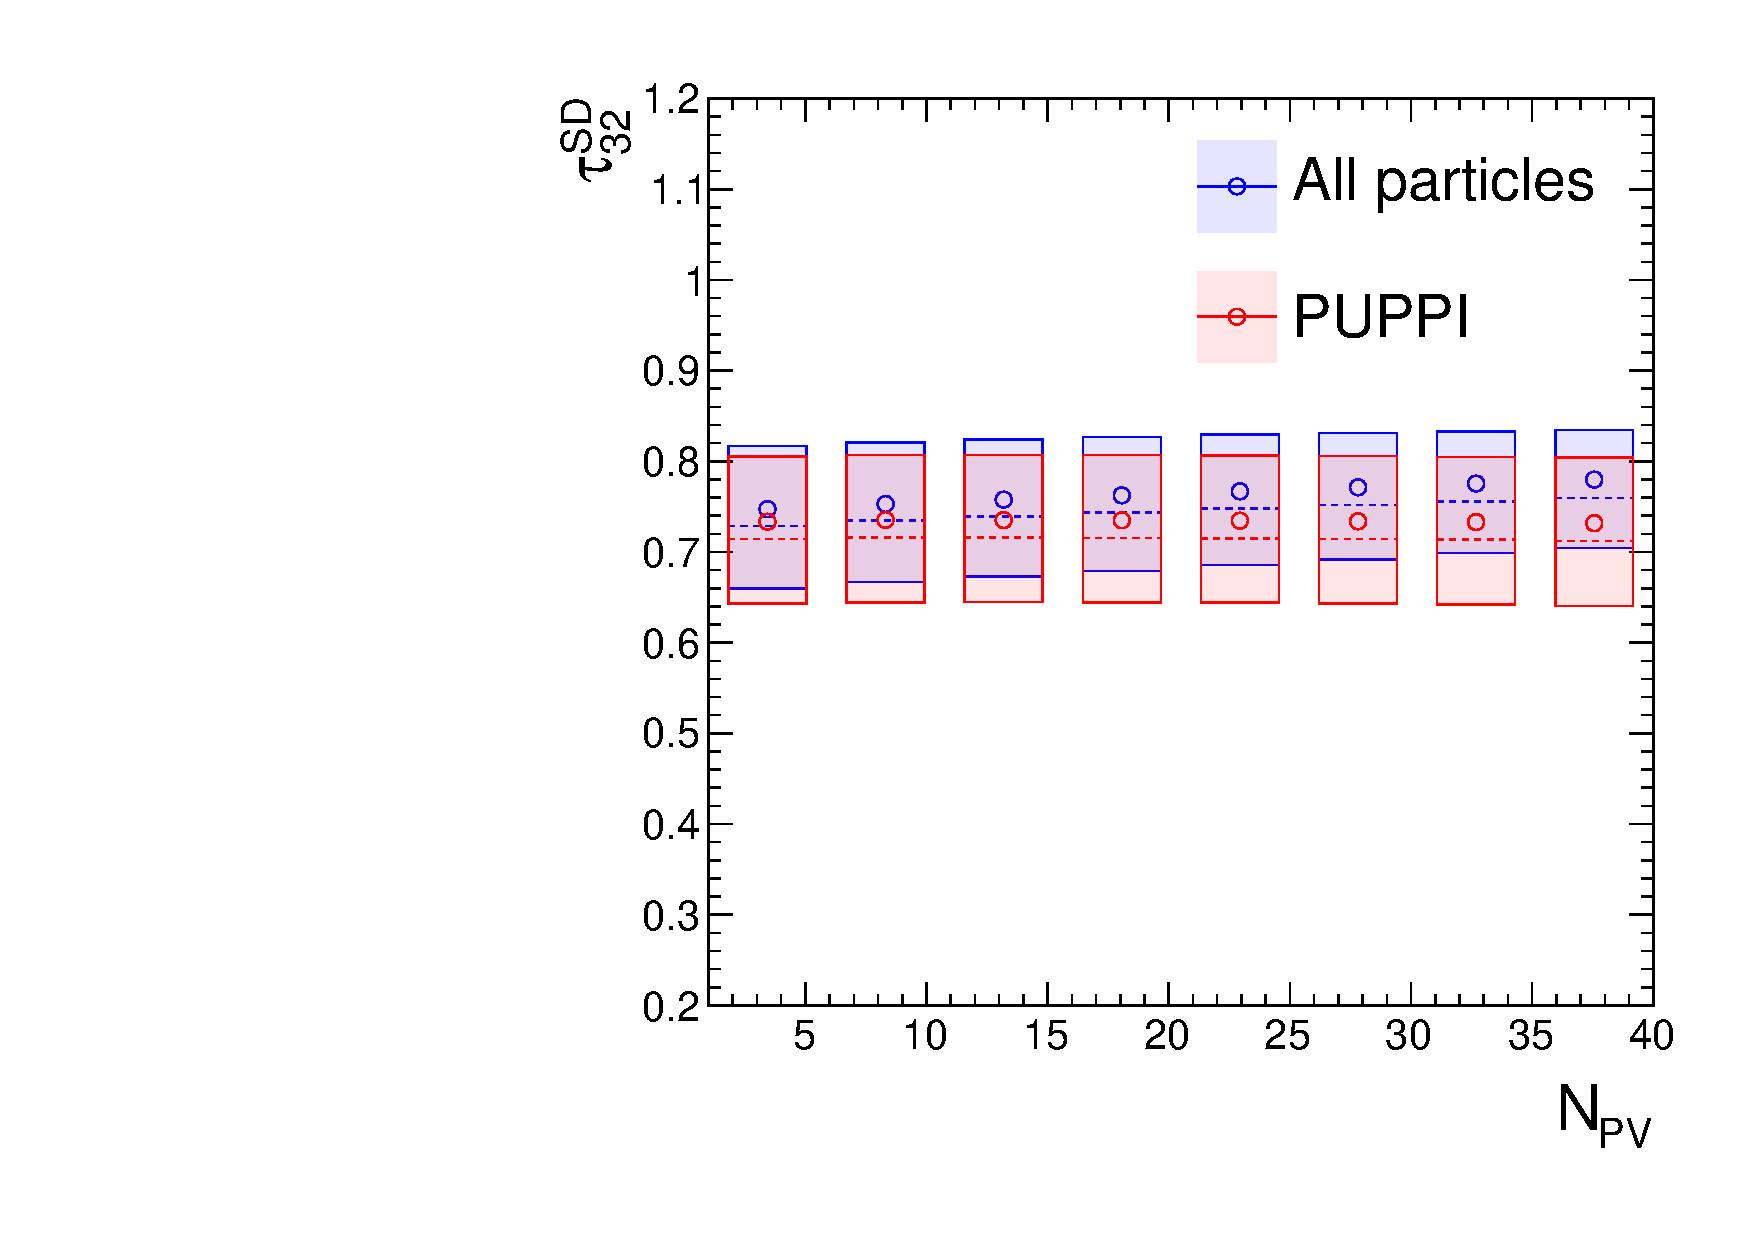
\includegraphics[width=\textwidth]{figures/toptagging/gen/npv_clf_Tau32SD_QCD.pdf}
            \caption{$\tau_{32}^\SD$, LQG}
        \end{subfigure}
        \begin{subfigure}[t]{0.35\textwidth}
            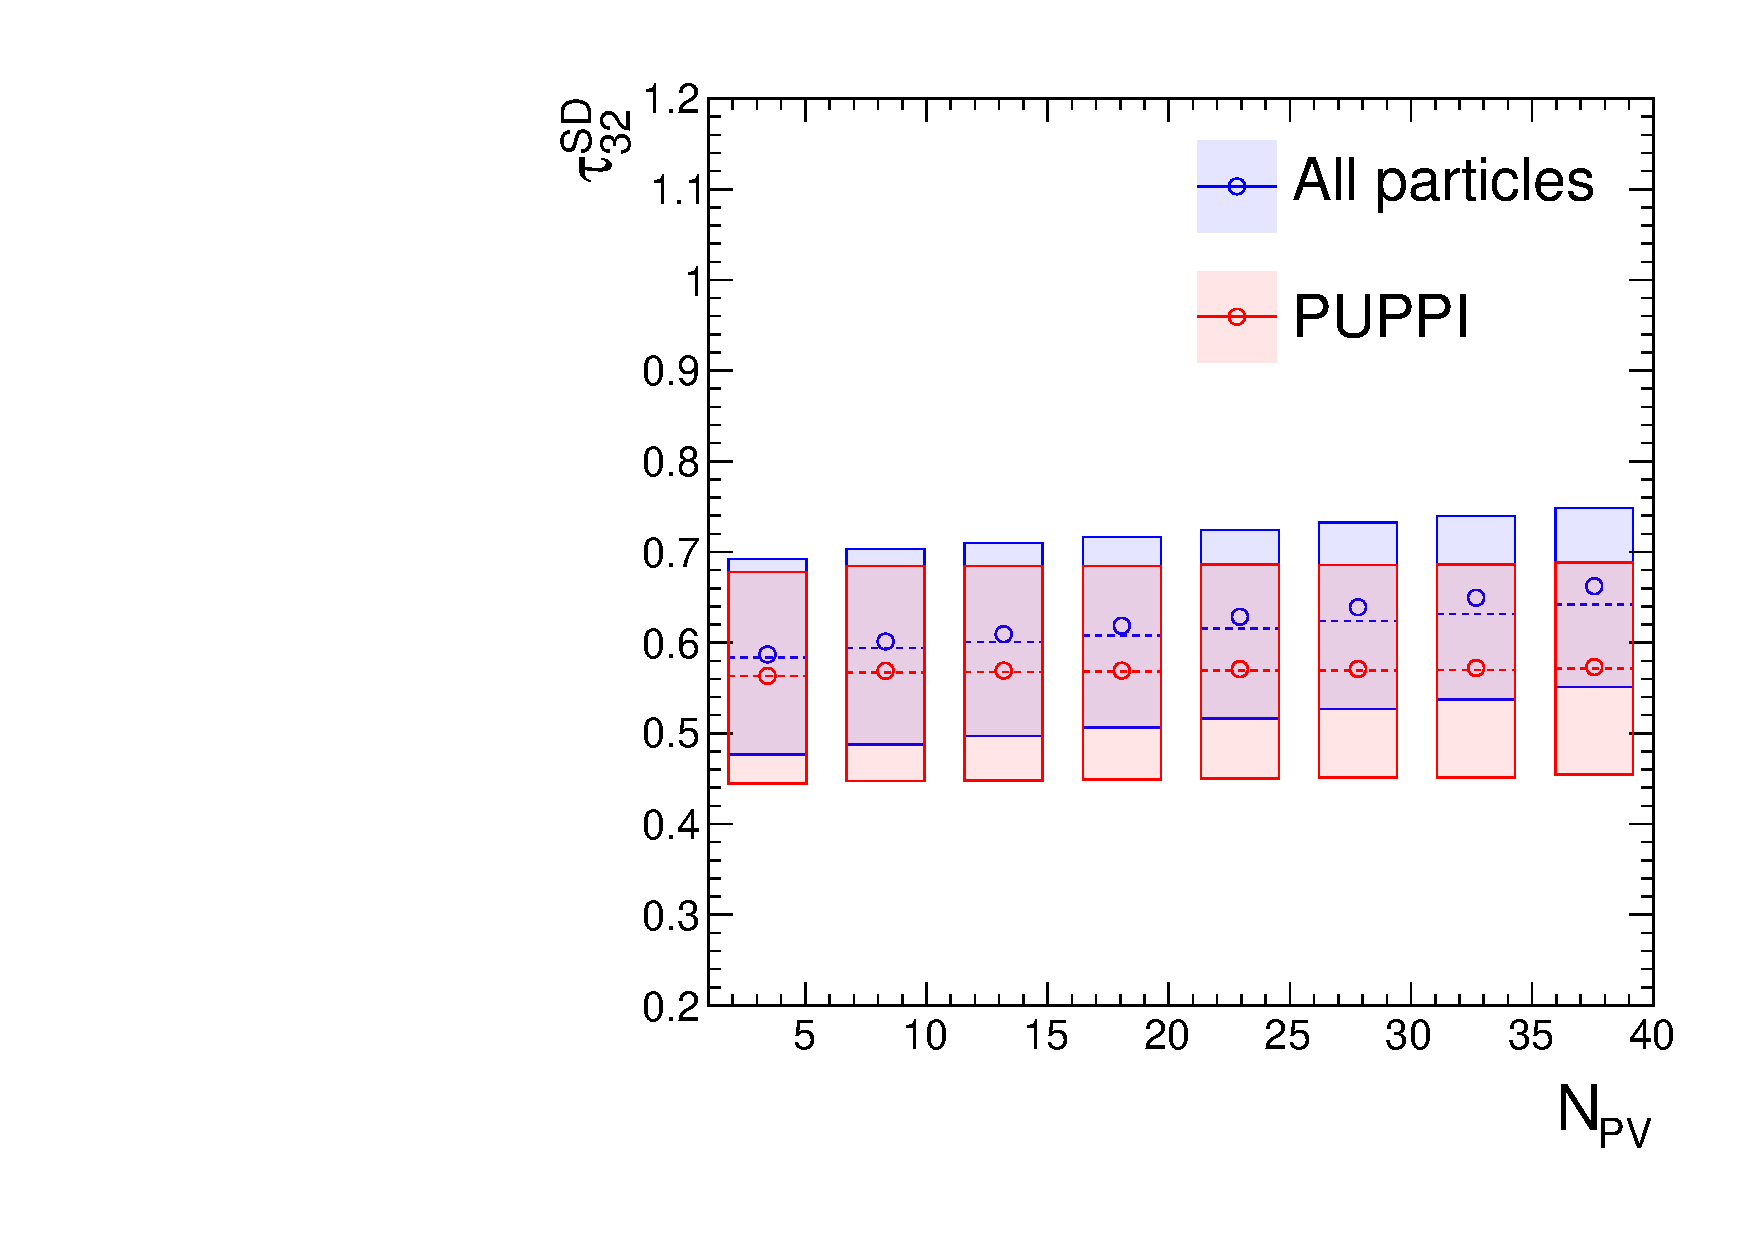
\includegraphics[width=\textwidth]{figures/toptagging/gen/npv_clf_Tau32SD_ZpTT_lo.pdf}
            \caption{$\tau_{32}^\SD$, Top}
        \end{subfigure}
        \caption{Stability of two CA15 jet observables (described in Section~\ref{sec:jets:id}) as a function of $N_\mathrm{PV}$.
            The median (mean) of each \NPV~bin is represented by an open circle (dashed line), while the $[25\%,75\%]$ percentile range is shown with a box.}
        \label{fig:jets:puppi}
    \end{center}
\end{figure}


\section{Identification}
\label{sec:jets:id}

Having \emph{reconstructed} the candidate top quark jets, we turn to the problem of \emph{identifying} which CA15 jets originate from top quarks as opposed to light $q/g$ hadronization. 
As indicated in Figure~\ref{fig:jets:caak}, the jet mass is a powerful observable, but top (LQG) jets do not necessarily have a mass of $m_t$ ($m_q,m_g\sim 0$). 
While some of this discrepancy is caused by mismeasurement of the jet energy scale (Chapter~\ref{sec:cms}), a substantial fraction originates from extra radiation being absorbed into the jet.
These extra particles arise from pile-up (although this is accounted for by PUPPI), initial state radiation, and underlying event.
Many algorithms exist to ``groom'' such particles from a jet after it has been clustered; here, we will discuss and use the soft drop (SD) method~\needcite.
SD functions by traversing the CA clustering history (a binary tree) in reverse and removing subjets (i.e. branches) of the clustering tree that are deemed to be too soft or wide-angled.
More formally, at each node in the clustering tree, the softer subjet of the node will be removed if it satisfies the condition:
\begin{equation}
    \frac{\min(p_\mathrm{T,1},p_\mathrm{T,2})}{p_\mathrm{T,1}+p_\mathrm{T,2}} < 
    \left(\frac{\Delta R_{12}}{R}\right)^\beta
\end{equation}
where $p_\mathrm{T,i}$ refers to the \pt~of the $i$-th subjet of the node; $\Delta R_{12}$ is the $\Delta R$-distance between the two subjet; and $R$ and $\beta$ are tunable parameters. 
This process starts at the root node of the clustering tree (i.e. the whole jet) and proceeds iteratively to the leaves (i.e. individual particles).
This condition is satisfied if the two subjets are very far apart (assuming $\beta \geq 0)$ or if the splitting is very asymmetric in momentum. 
We define the ``SD subjets'' (or where clear, simply ``subjets'') of a jet to be the two branches of the root node, after branches failing the SD condition have been removed. 
The particles remaining after this grooming procedure are combined to make the ``groomed'' or SD jet. 

We then define $m_\mathrm{SD}$ as the mass of the SD jet. 
Observables may also be defined in terms of the groomed or ungroomed jet. 
Figure~\ref{fig:jets:msd} compares the ungroomed and groomed mass distributions in top and LQG jets, as a function of jet momentum. 
It is immediately clear that grooming provides (a) a sharper mass peak in top jets at $m_t$ and (b) a smoothly falling mass distribution in LQG jets that goes to 0.
Furthermore, SD ensures the stability of the mass distribution as a function of jet \pt, especially in LQG jets.
For these reasons, $m_\mathrm{SD}$ will be our standard definition of jet mass. 


\begin{figure}[]
    \begin{center}
        \begin{subfigure}[t]{0.35\textwidth}
            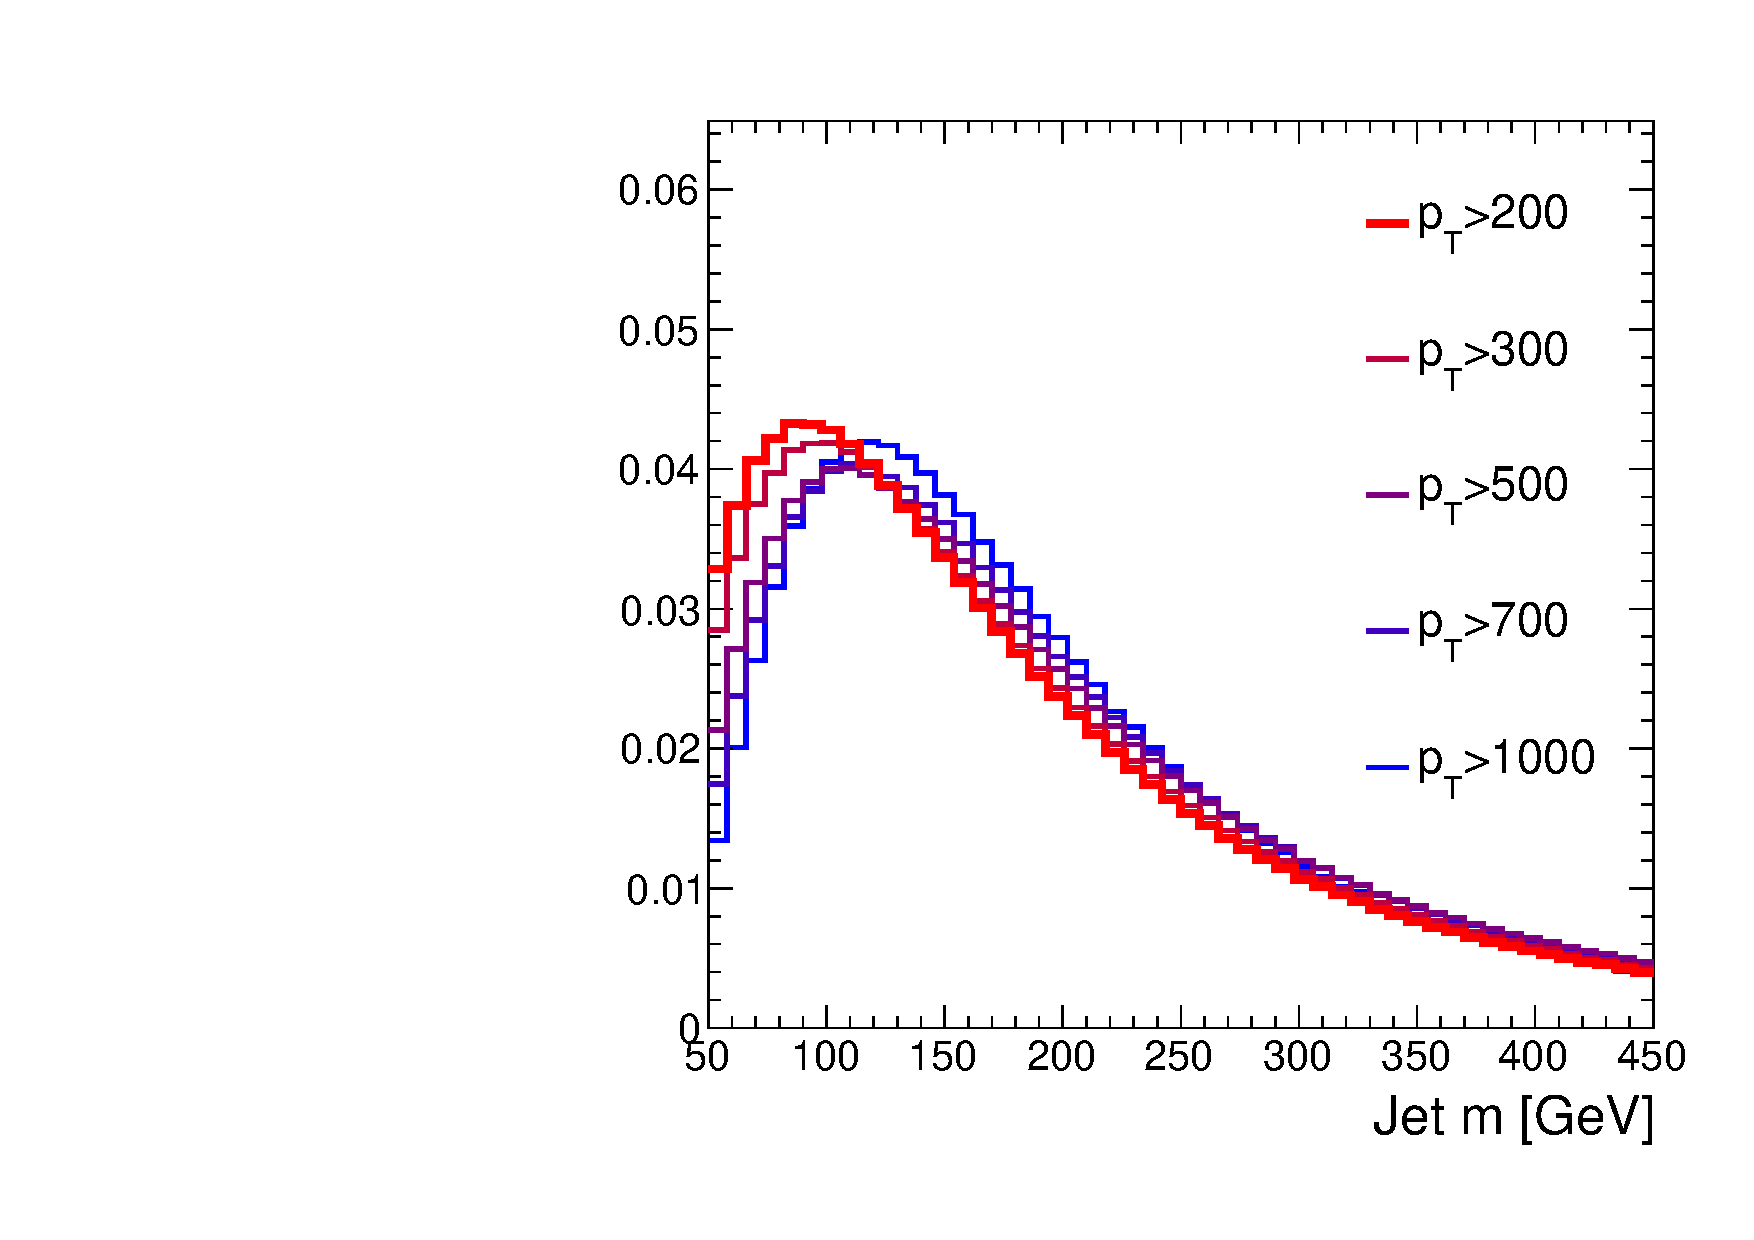
\includegraphics[width=\textwidth]{figures/toptagging/gen/norm_clf_M_QCD.pdf}
            \caption{Ungroomed, LQG}
        \end{subfigure}
        \begin{subfigure}[t]{0.35\textwidth}
            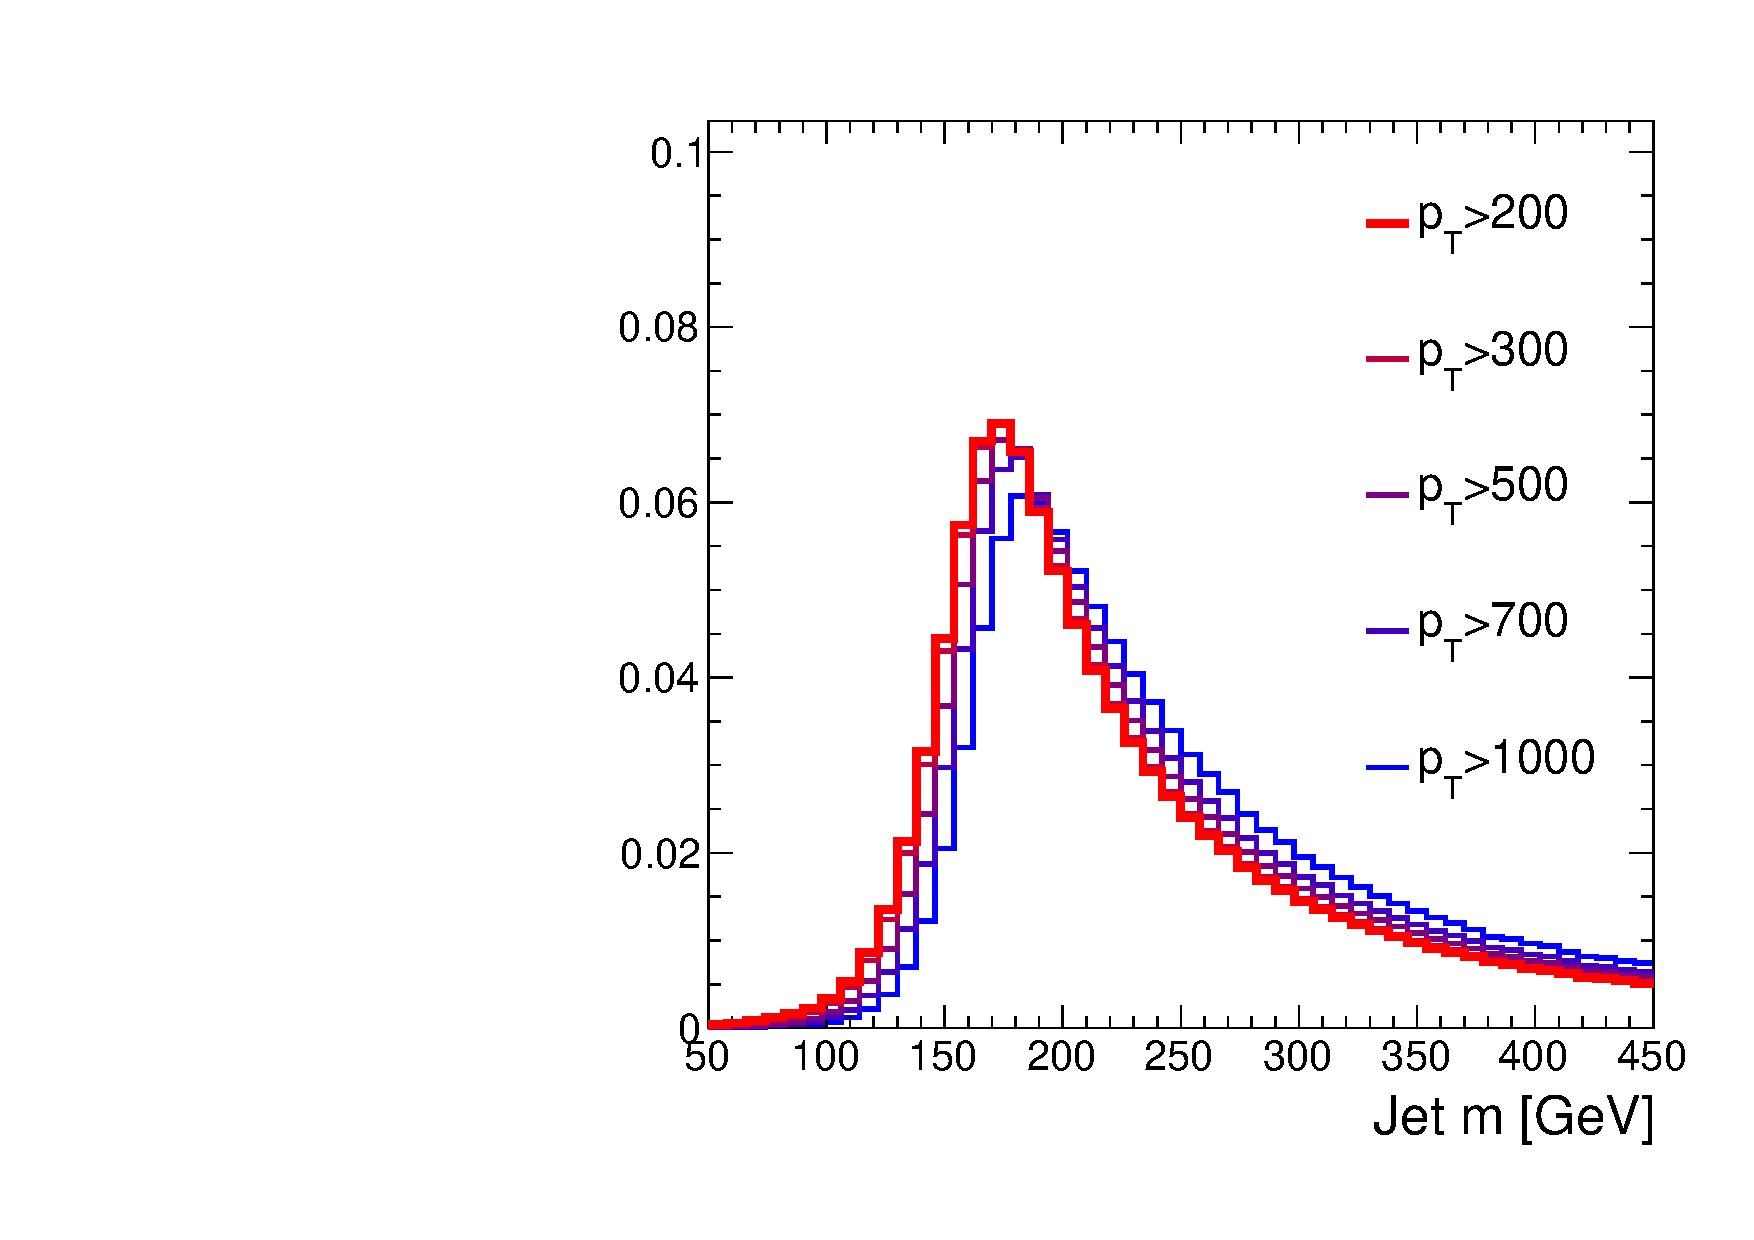
\includegraphics[width=\textwidth]{figures/toptagging/gen/norm_clf_M_ZpTT_lo.pdf}
            \caption{Ungroomed, Top}
        \end{subfigure}
        \begin{subfigure}[t]{0.35\textwidth}
            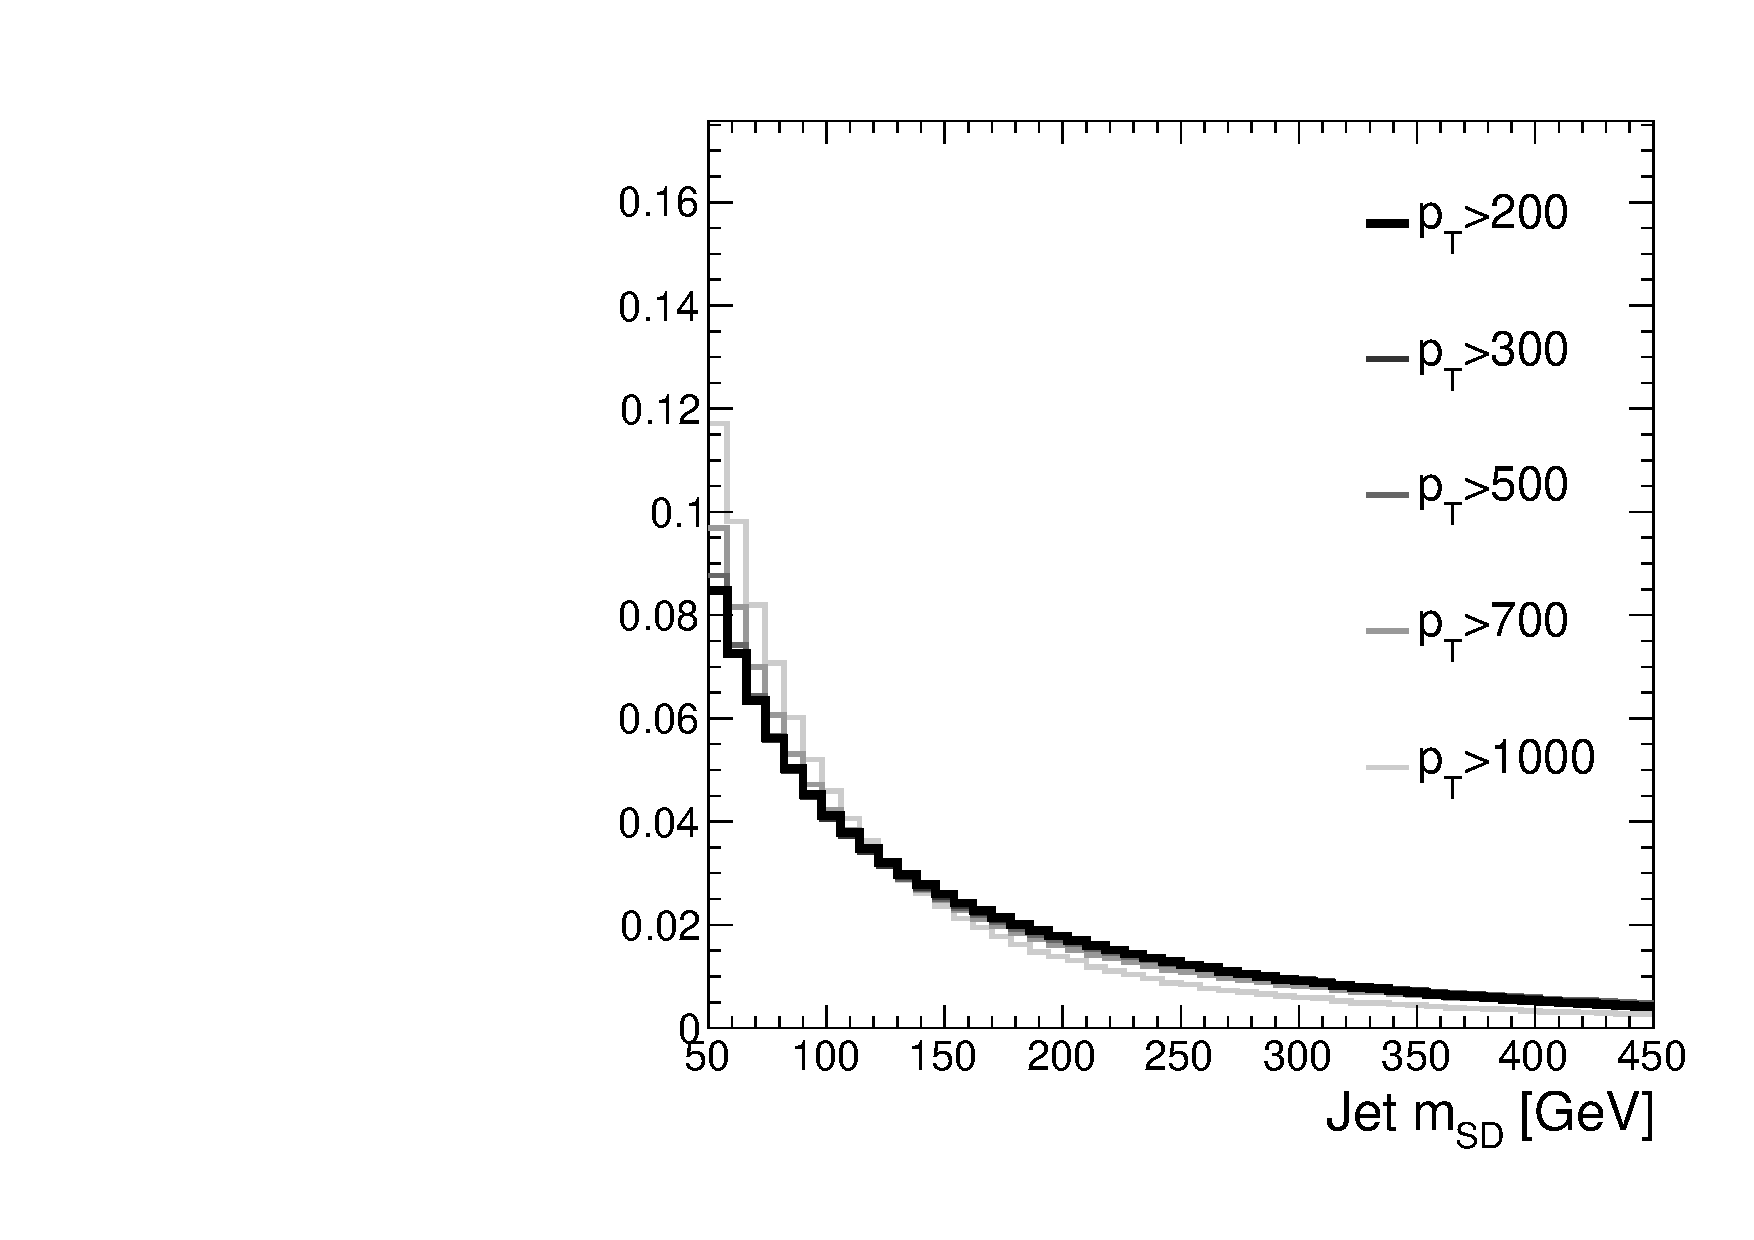
\includegraphics[width=\textwidth]{figures/toptagging/gen/norm_clf_MSD_QCD.pdf}
            \caption{SD, LQG}
        \end{subfigure}
        \begin{subfigure}[t]{0.35\textwidth}
            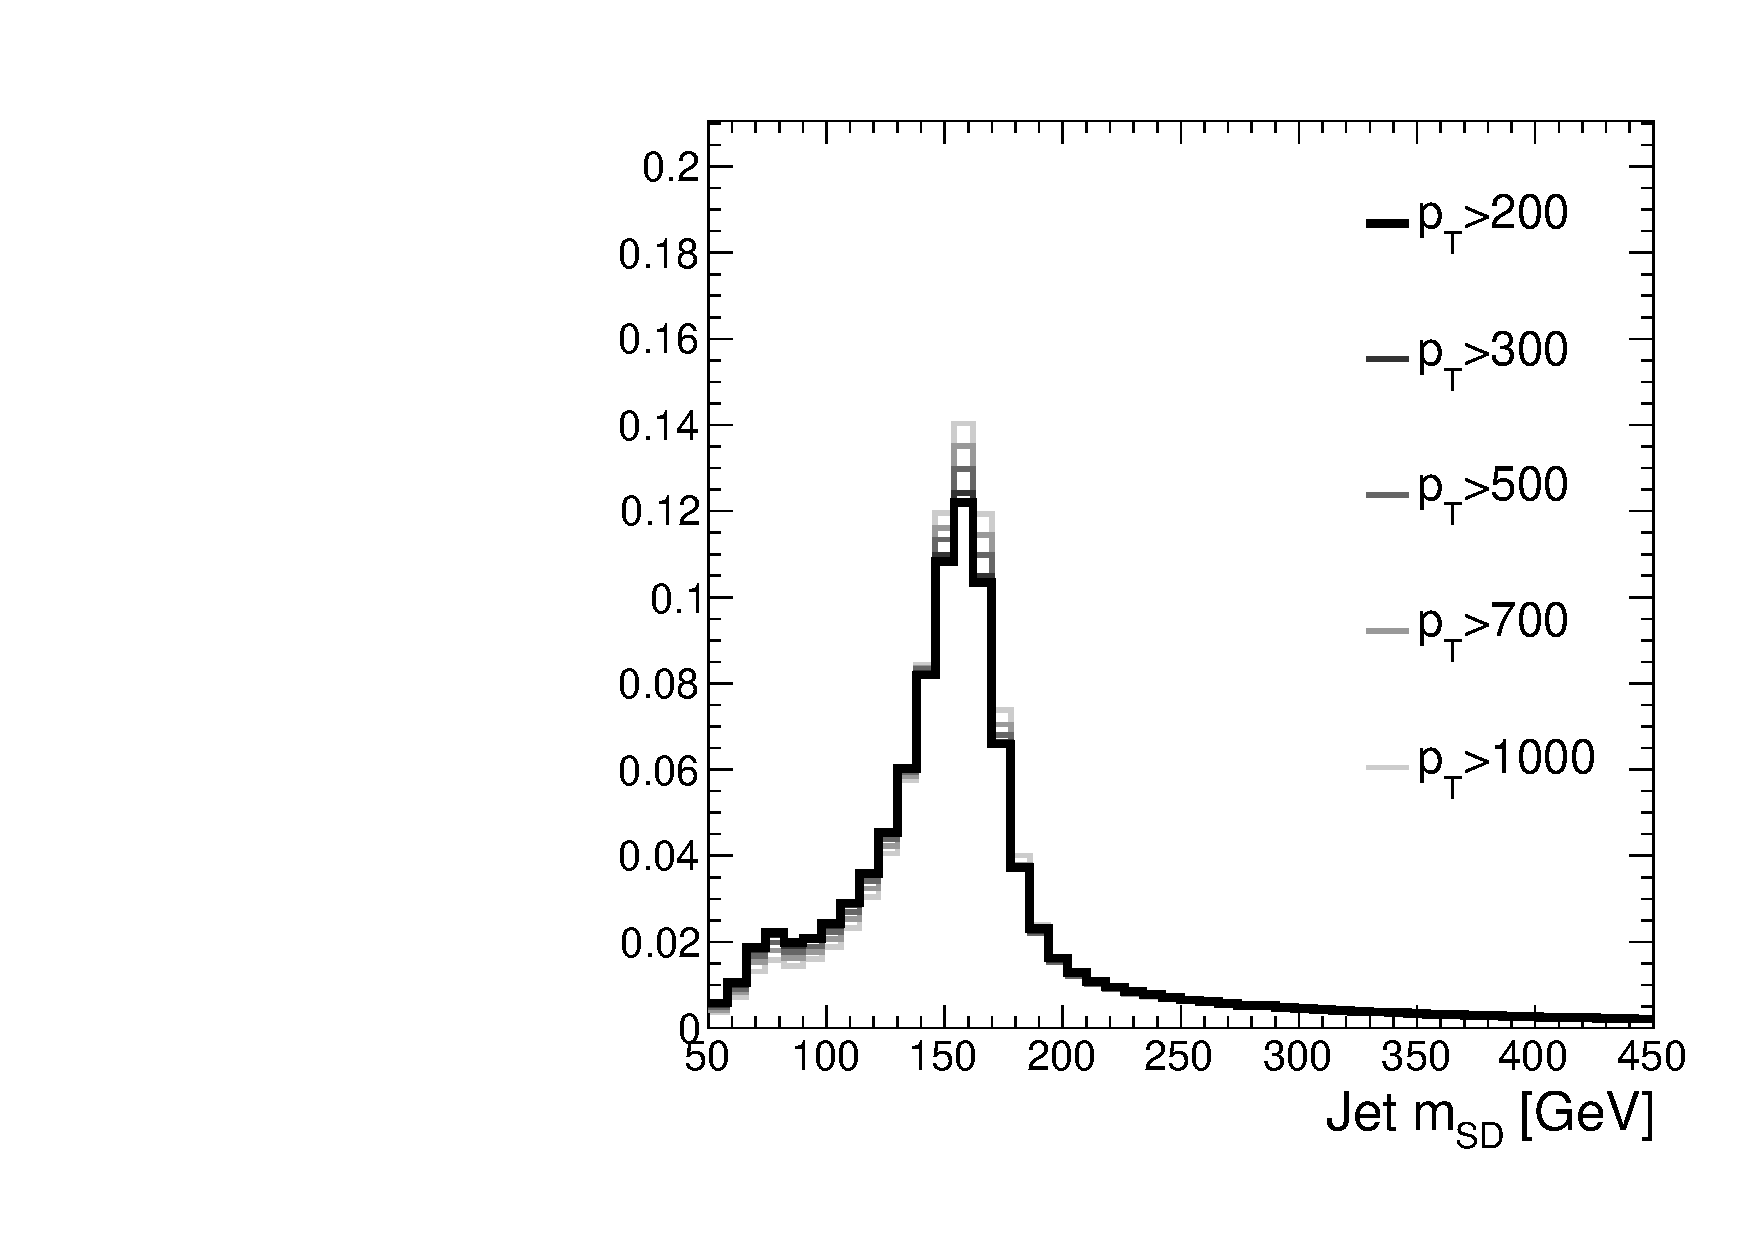
\includegraphics[width=\textwidth]{figures/toptagging/gen/norm_clf_MSD_ZpTT_lo.pdf}
            \caption{SD, Top}
        \end{subfigure}
        \caption{Distribution of ungroomed and groomed jet mass in CA15 jets originating from LQG or hadronic top decays.
                 The multiple histograms represent increasingly stringent \pt~requirements on the parton that initiates the jet.}
        \label{fig:jets:msd}
    \end{center}
\end{figure}

\subsection{Substructure}

A substructure observable is any function of a jet's constituents that is sensitive to the multi-pronged structure of a heavy resonance decay. 
In addition to jet mass and $b$-tagging, substructure is used to reject LQG jets as top decay candidates. 

\subsubsection{$N$-subjettiness}

The $N$-subjettiness ($\tau_N$) is a measure of the compatibility of a jet with an $N$-axis hypothesis~\needcite.
It is defined as:
\begin{equation}
    \tau_N = \frac{\sum_{i\in\mathrm{jet}} p_{\mathrm{T},i} \min\{\Delta R_{ia} | a\in A\}}{\sum_{i\in\mathrm{jet}} p_{\mathrm{T},i} R}
\end{equation}
where $R=1.5$ (the jet radius); $\Delta R_{ia}$ is the $\Delta R$ distance between the particle $i$ and the axis $a$; and $A$ is a set of $N$ axes. 
Ideally, $A$ would be defined to be the set of axes that minimize $\tau_N$ for each jet, but this minimization problem is computationally difficult.  
Instead, the exclusive \kt~algorithm is used to partition the jet's constituents into $N$ subjets (NB: these are not the SD subjets discussed above).
Since the \kt~distance metric is proportional to $\nicefrac{\Delta R^2}{R^2}$, this approximates the ideal minimization.
The set of axes $A$ is taken to be the directions of the $N$ \kt~subjets. 
A small $\tau_N$ indicates a high degree of compatibility with the $N$-axis hypothesis.
Therefore, we expect a 3-pronged (e.g. top) jet to satisfy $\tau_3 \ll \tau_2$, whereas a 1-pronged (e.g. LQG) jet should satisfy $\tau_3 \lesssim \tau_2$ (for optimal choice of $A$, $N>M \Rightarrow \tau_{N} \leq \tau_{M}$ for any jet). 
Correspondingly, we take $\tau_{32} \equiv \nicefrac{\tau_3}{\tau_2}$ to be the tagging observable. 

Figure~\ref{fig:jets:tau32} shows the distribution of $\tau_{32}$.
As with jet mass, we may calculate $\tau_{32}$ either on the whole jet or on the groomed (SD) jet.
The discrimination between top and LQG jets is similar in both cases, but as Figure~\ref{fig:jets:msdtau} demonstrates, $\tau_{32}^\SD$ has the weaker correlation with $m_\SD$ in LQG jets. 
This feature will be critical to validate any tagger in data, as described in Section~\ref{sec:jets:sf}.

\begin{figure}[]
    \begin{center}
        \begin{subfigure}[t]{0.32\textwidth}
            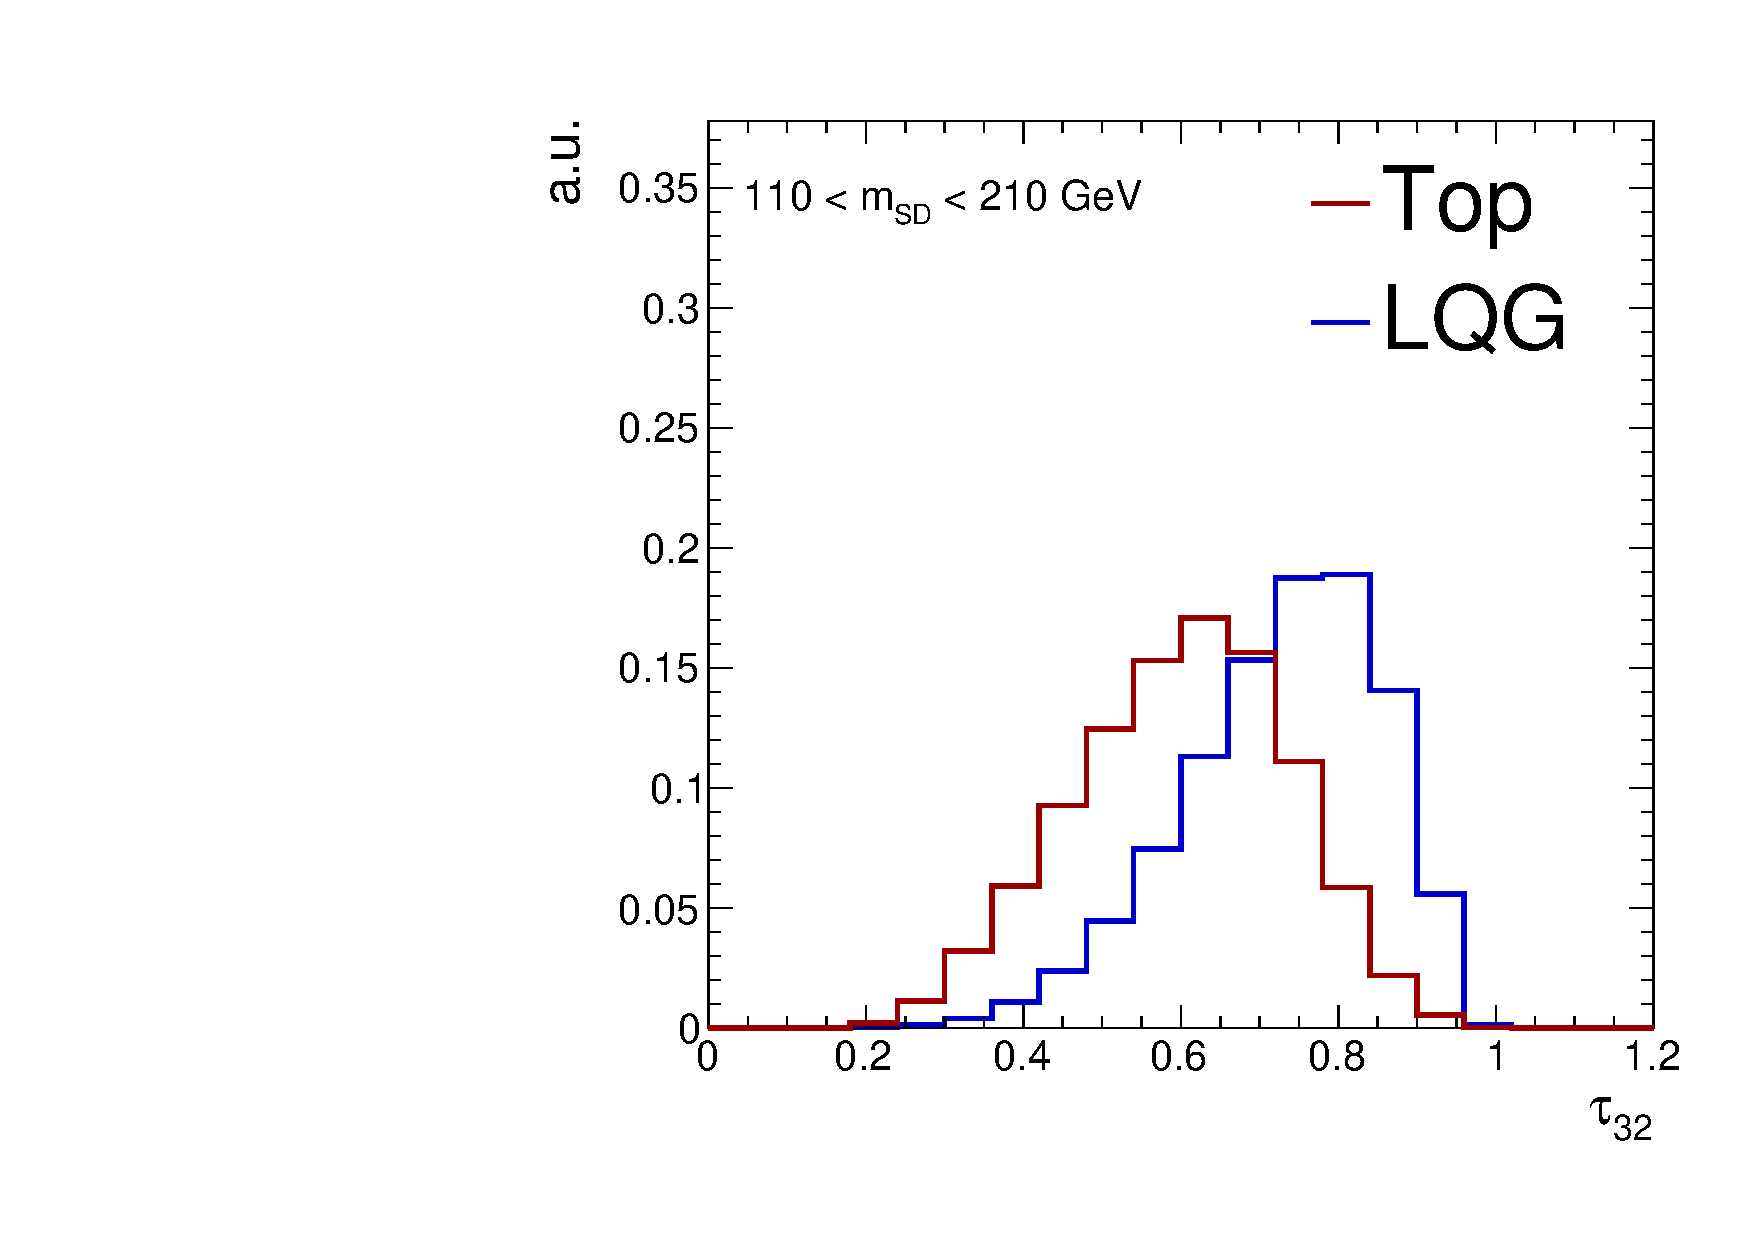
\includegraphics[width=\textwidth]{figures/toptagging/shapes/mass_fjTau32.pdf}
            \caption{}
        \end{subfigure}
        \begin{subfigure}[t]{0.32\textwidth}
            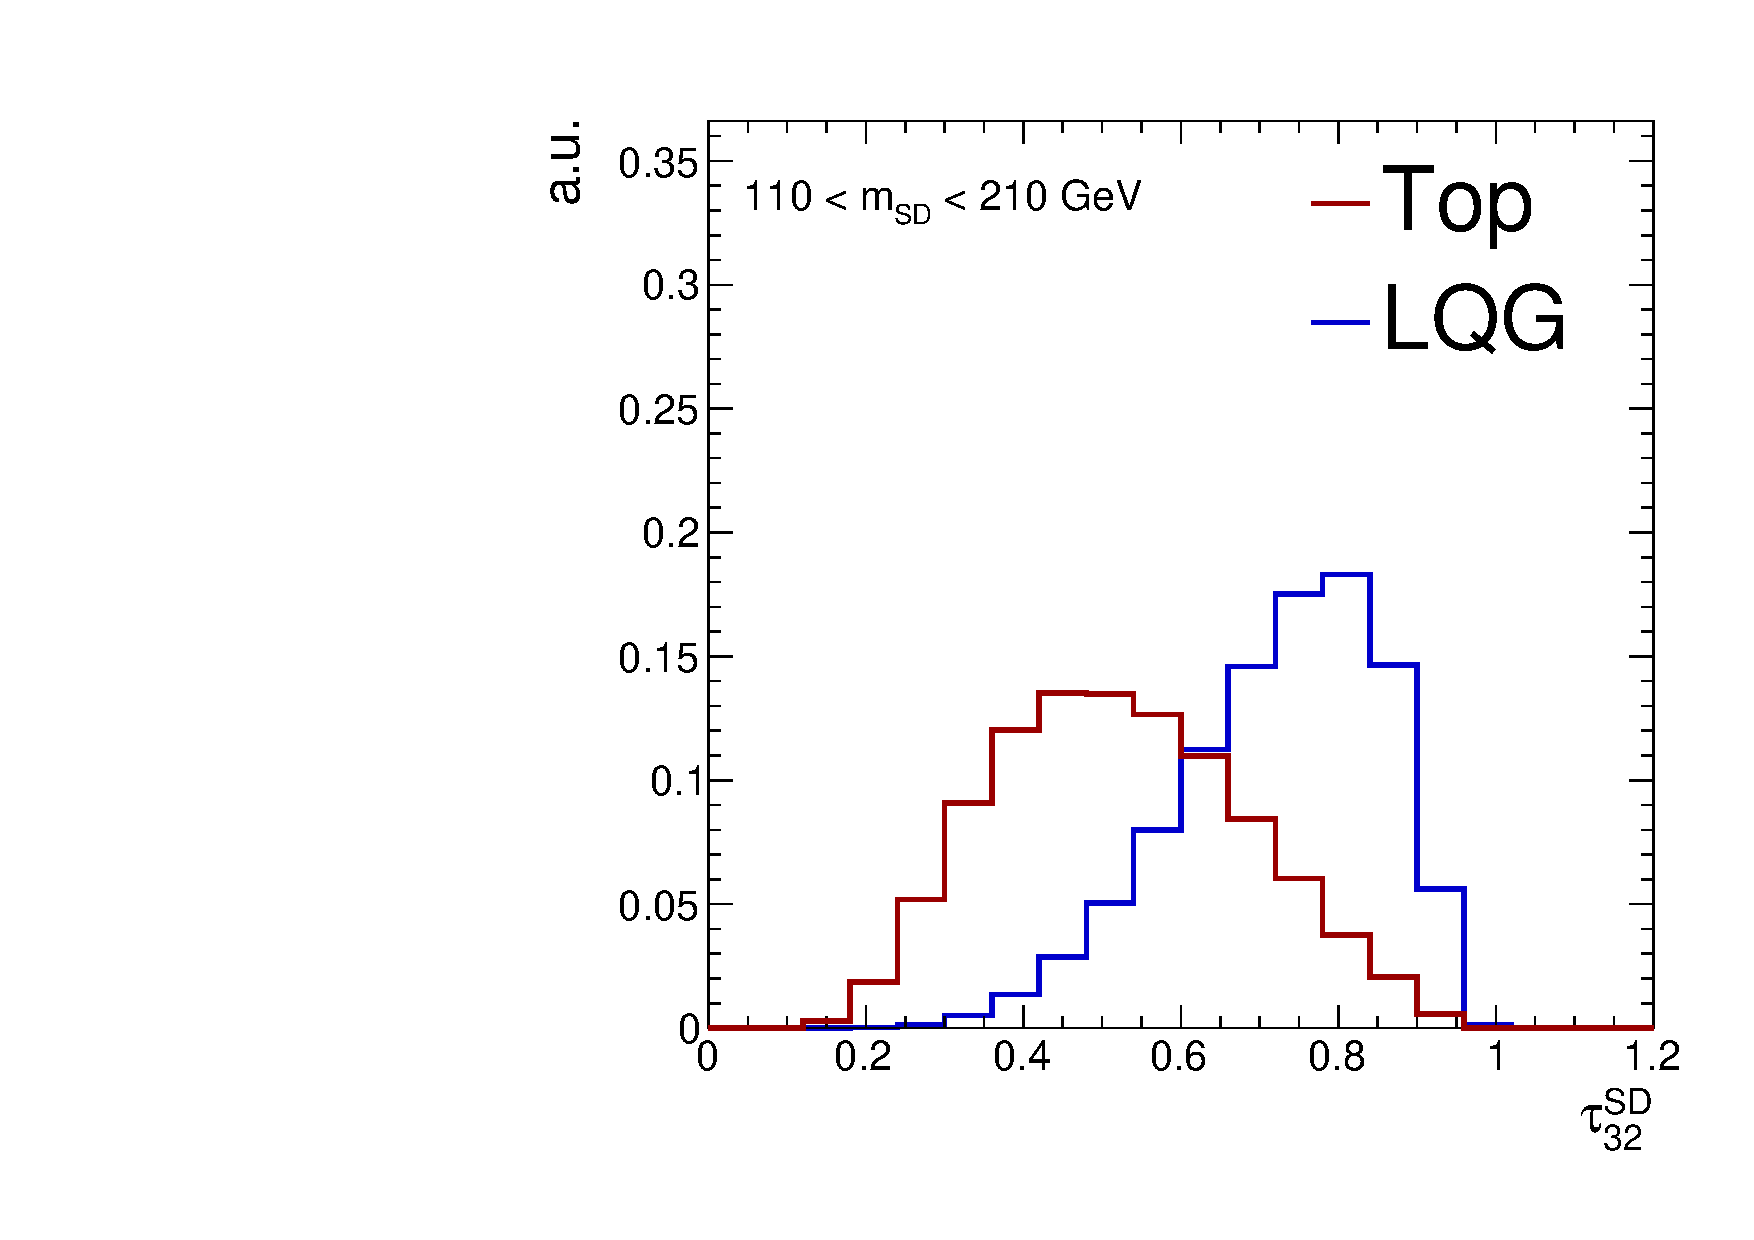
\includegraphics[width=\textwidth]{figures/toptagging/shapes/mass_fjTau32SD.pdf}
            \caption{}
        \end{subfigure}
        \begin{subfigure}[t]{0.32\textwidth}
            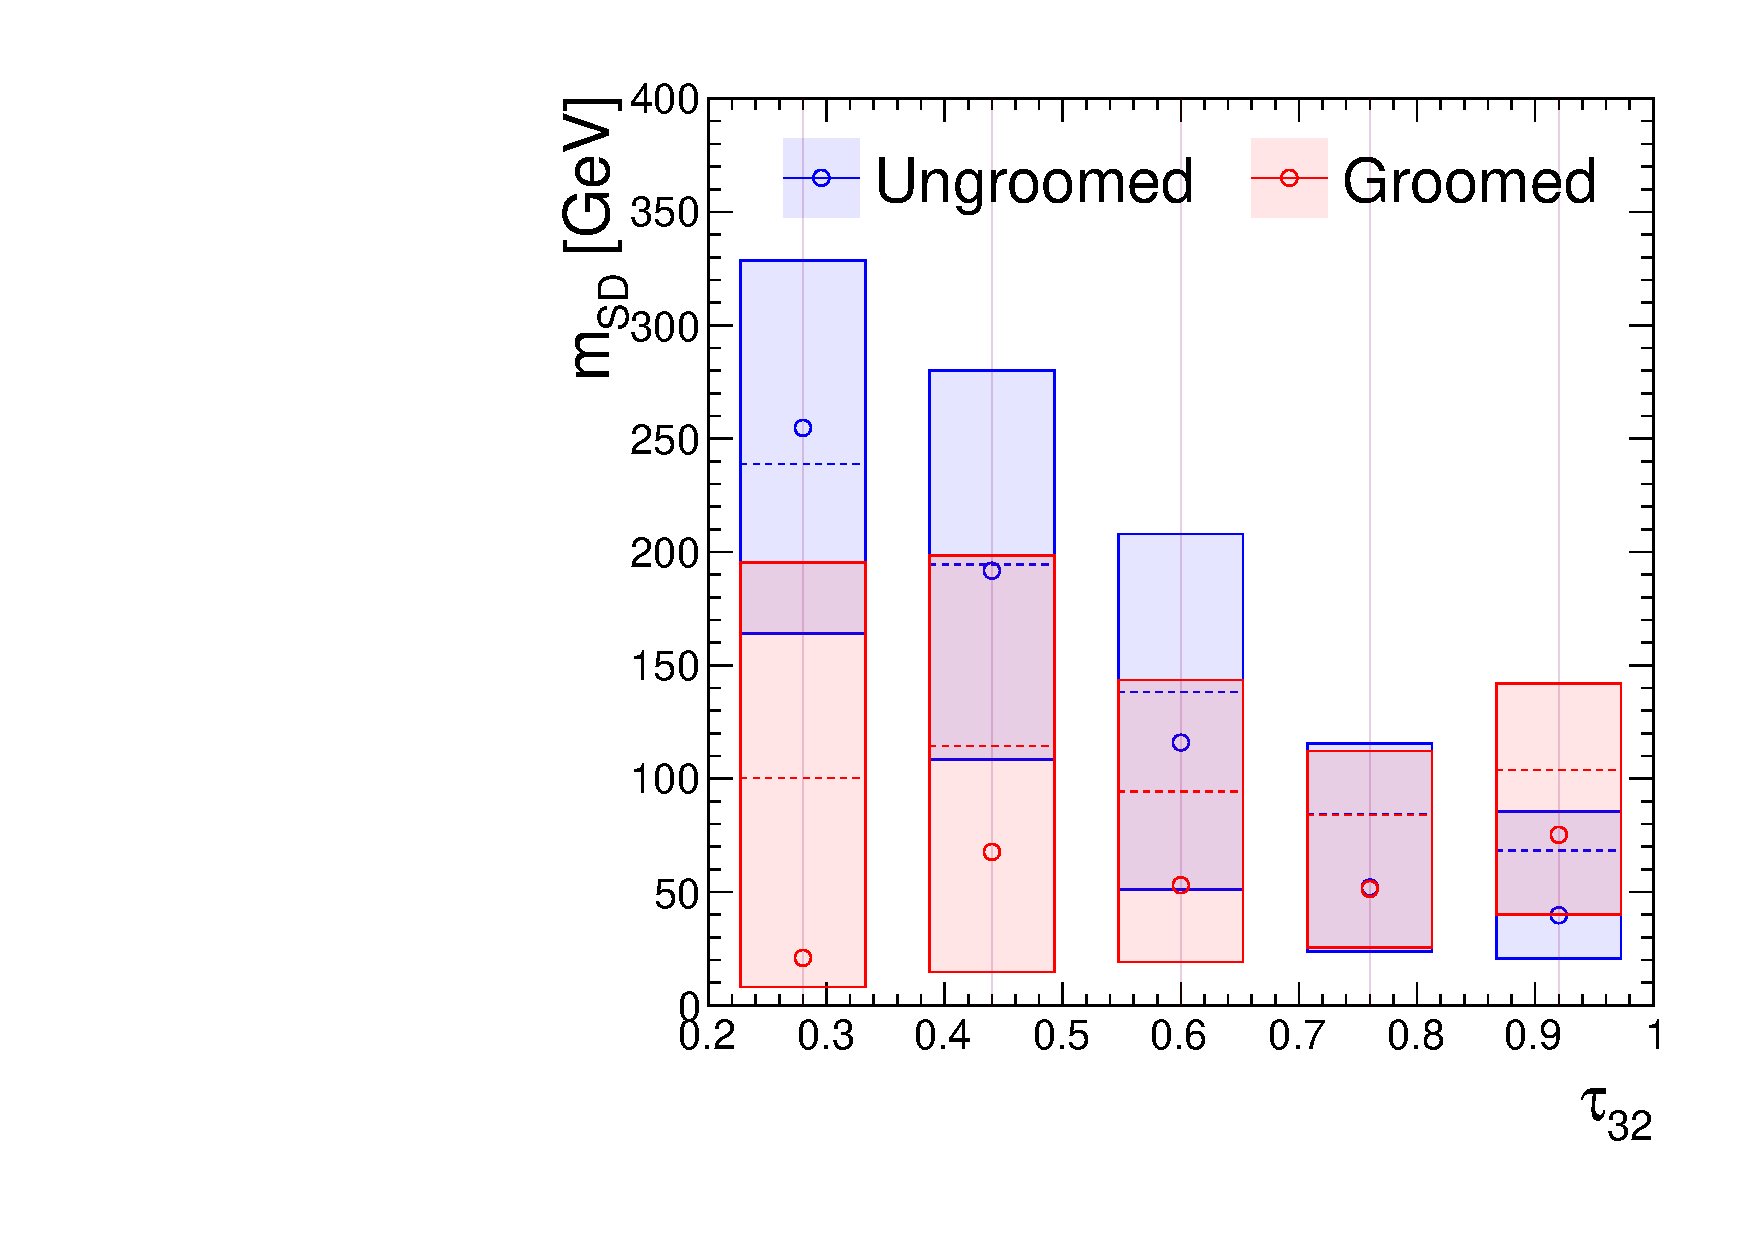
\includegraphics[width=\textwidth]{figures/toptagging/gen/msdtau_QCD.pdf}
            \caption{}
            \label{fig:jets:msdtau}
        \end{subfigure}
        \caption{Shape of ungroomed (left) and groomed (center) $\tau_{32}$ distributions in top and LQG jets, with a mass selection consistent with $m_t$. 
                 Right: the correlation between $\tau_{32}$ and $m_\SD$ in LQG jets, comparing groomed and ungroomed jets. 
                 }
        \label{fig:jets:tau32}
    \end{center}
\end{figure}

\subsubsection{\HTT}
% https://arxiv.org/pdf/1503.05921.pdf

The \HTT~algorithm de-clusters the jet into many subjets and attempts to reconstruct the $W$ and $t$ decay products out of these subjets~\needcite.
The computation of the tagging variable \frec~can be simplified into three steps (a more detailed description is found in the appendix of Reference~\needcite):
\begin{enumerate}
    \item Compute subjets of the CA15 jet. This is done in a fashion similar to the SD subjets discussed above, but instead of taking the two subjets of the root node, the tree is traversed until some lower \pt~bound is crossed.
    \item Test all triplet combinations of the found subjets and define the $m_{123}$ as the groomed mass of the trijet system. 
    \item Choosing the triplet most consistent with a 3-body top decay (see Equation 12 in Reference~\needcite), define:
        \begin{equation}
            \frec = \min_{0\leq i < j \leq 2} \left|
            \frac{\nicefrac{m_{ij}}{m_{123}}}{\nicefrac{m_W}{m_t}} - 1\right|
        \end{equation}
        where the indices $i,j$ index elements of the selected triplet. 
\end{enumerate}
Figure~\ref{fig:jets:htt} shows the distribution of the selected $m_{123}$ and $\frec$, although we will only use the latter as a tagging observable. 
Note that we do not define distinct groomed and ungroomed versions of these observables, as grooming is intrinsically used in defining the subjets. 

\begin{figure}[]
    \begin{center}
        \begin{subfigure}[t]{0.35\textwidth}
            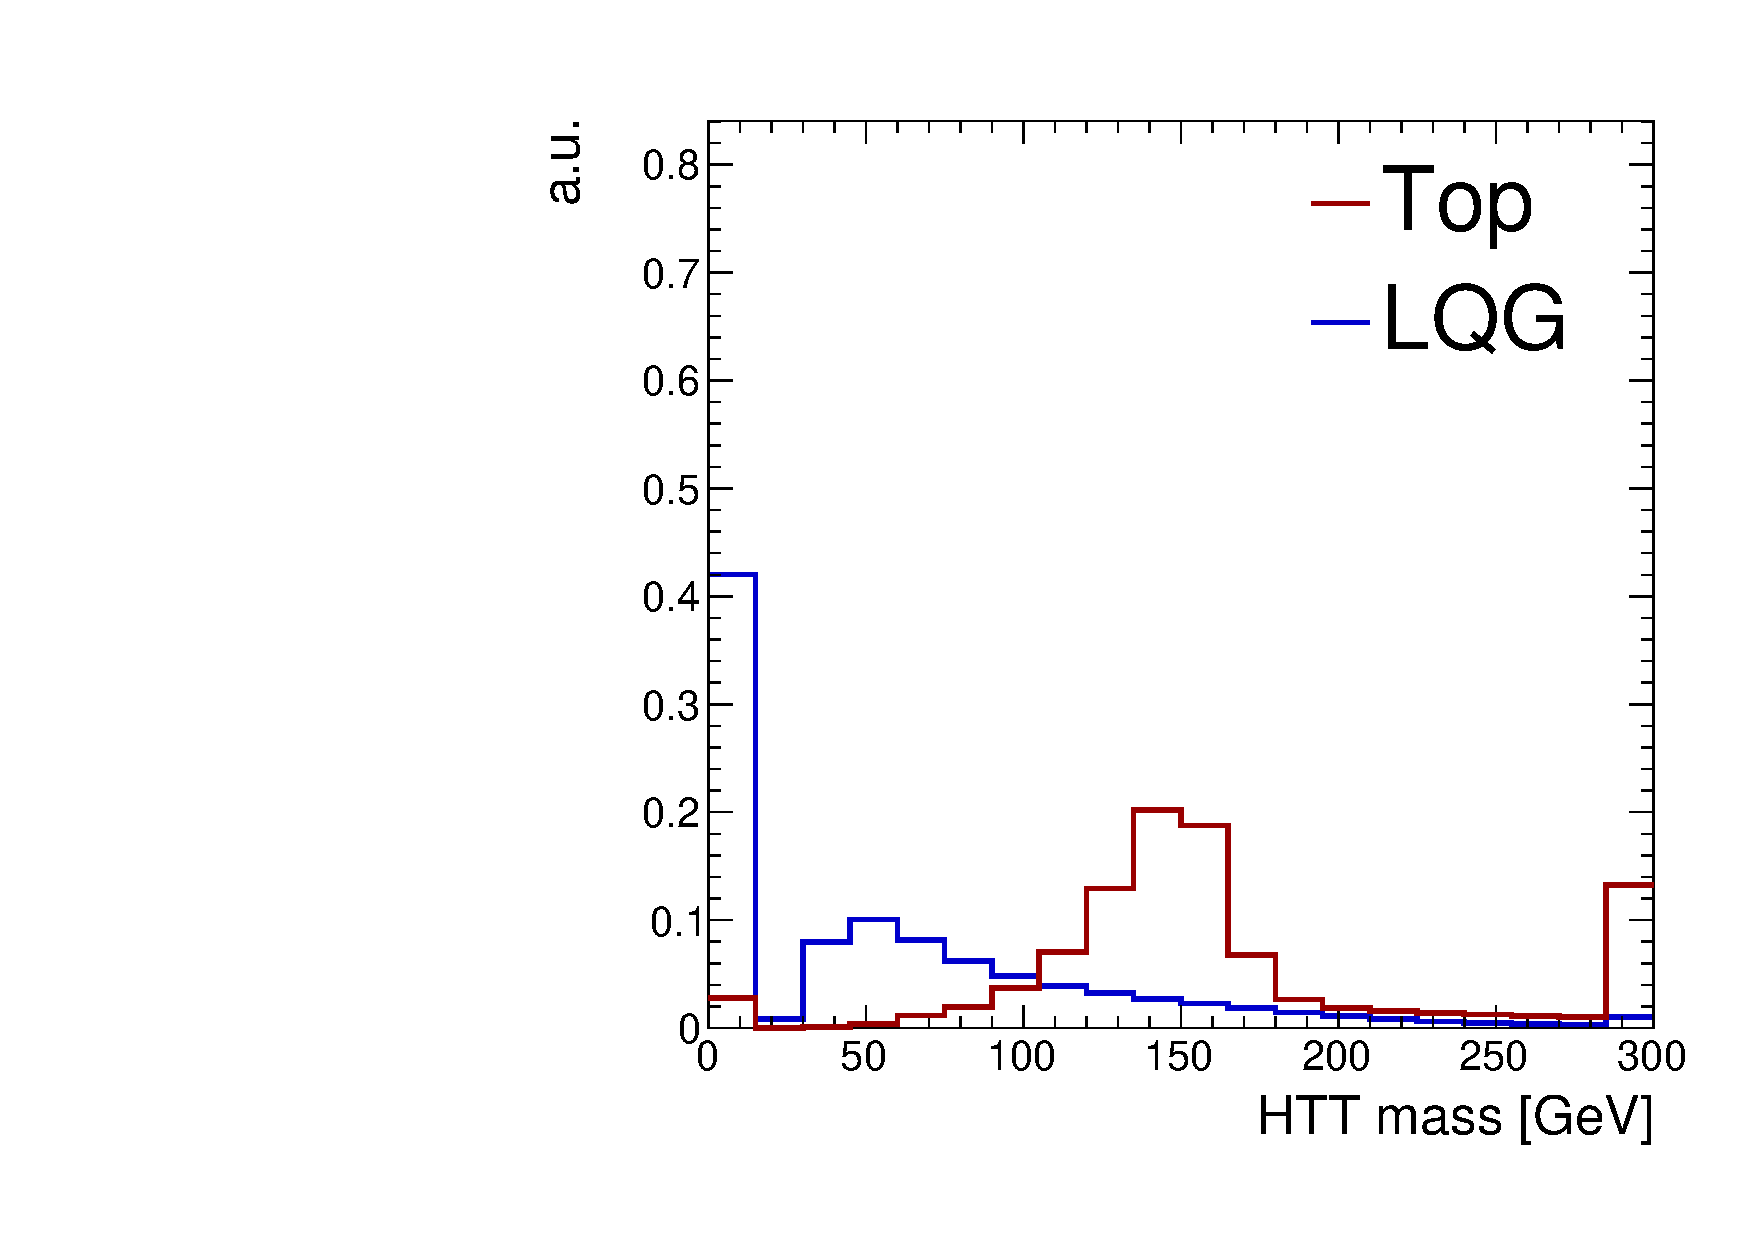
\includegraphics[width=\textwidth]{figures/toptagging/shapes/incl_fjHTTMass.pdf}
        \end{subfigure}
        \begin{subfigure}[t]{0.35\textwidth}
            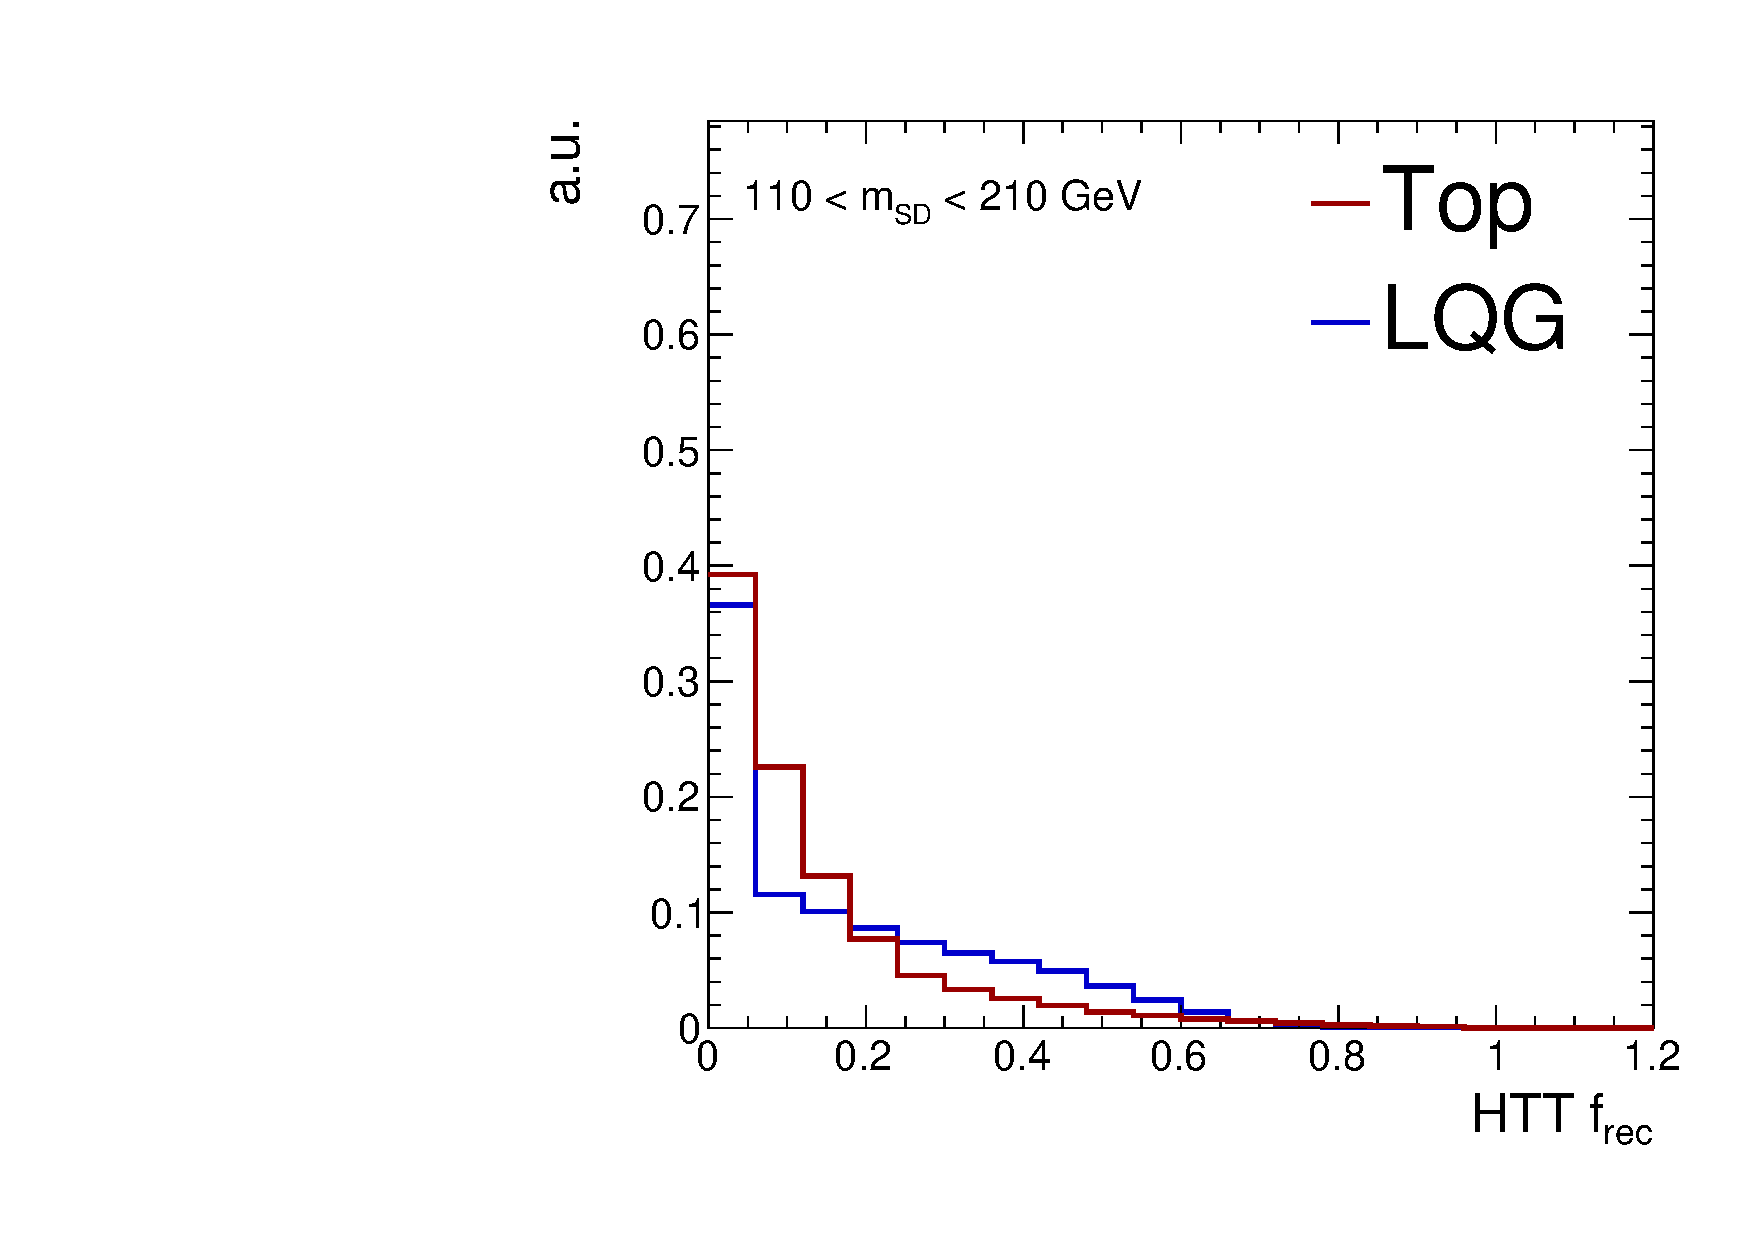
\includegraphics[width=\textwidth]{figures/toptagging/shapes/mass_fjHTTFRec.pdf}
        \end{subfigure}
        \caption{Shape of the $m_{123}$ and $\frec$ observables computed by the \HTT~algorithm. }
        \label{fig:jets:htt}
    \end{center}
\end{figure}

\subsubsection{Energy Correlation Functions}

Energy correlation functions measure the correlation of the positions of hard particles in a jet~\needcite. 
Heuristically, an $N$-point ECF is small if the hard particles can be grouped into fewer than $N$ prongs and large if they arise from $N$ or more prongs. 
An $N$-point ECF, with angular parameters $o$ and $\beta$, is defined as:
\begin{equation}
    e(o,N,\beta) \equiv 
    ~_o e_N^\beta = 
    \sum _{K\subset J, |K|=N} 
    \left[\prod_{i\in K} \frac{\pt^{(i)}}{\pt^{(J)}}\right] \times 
    \min\left\{ \prod_{i,j\in P} \Delta R_{ij}^\beta 
        ~\Big|~ P \subset (K^2 \backslash (k,k)),~|P|=o\right\}
\end{equation}
where $K^2\backslash(k,k)$ indicates all pairs of distinct particles in $K$. 
The proposed tagger in Reference~\needcite~is:
\begin{equation}
    N_3^{(\beta)} = \frac{e(2,4,\beta)}{(e(1,3,\beta))^2}
\end{equation}
Figure~\ref{fig:jets:n3} shows $N_3$ for various values of $\beta$; given our desire for stability as a function of jet \pt~and mass, we only consider ECFs computed on the SD jet. 
The discrimination power of this ECF ratio is roughly comparable to that of $\tau_{32}^\SD$. 
$N_3$ is motivated by the behavior of 3- and 4-point ECFs in top and LQG jets:
\begin{itemize}
    \item In top jets, $e(N=4) \ll e(N=3)$, since 3-point correlation functions are large in a 3-pronged jet
    \item In QCD jets, $e(N=3) \sim e(N=3)$, since both 3- and 4-point ECFs are weak in a 1-pronged jet
\end{itemize}
Therefore, taking the ratio $e(N=4)/e(N=3)$ constructs a useful observable. 

\begin{figure}[]
    \begin{center}
        \begin{subfigure}[t]{0.32\textwidth}
            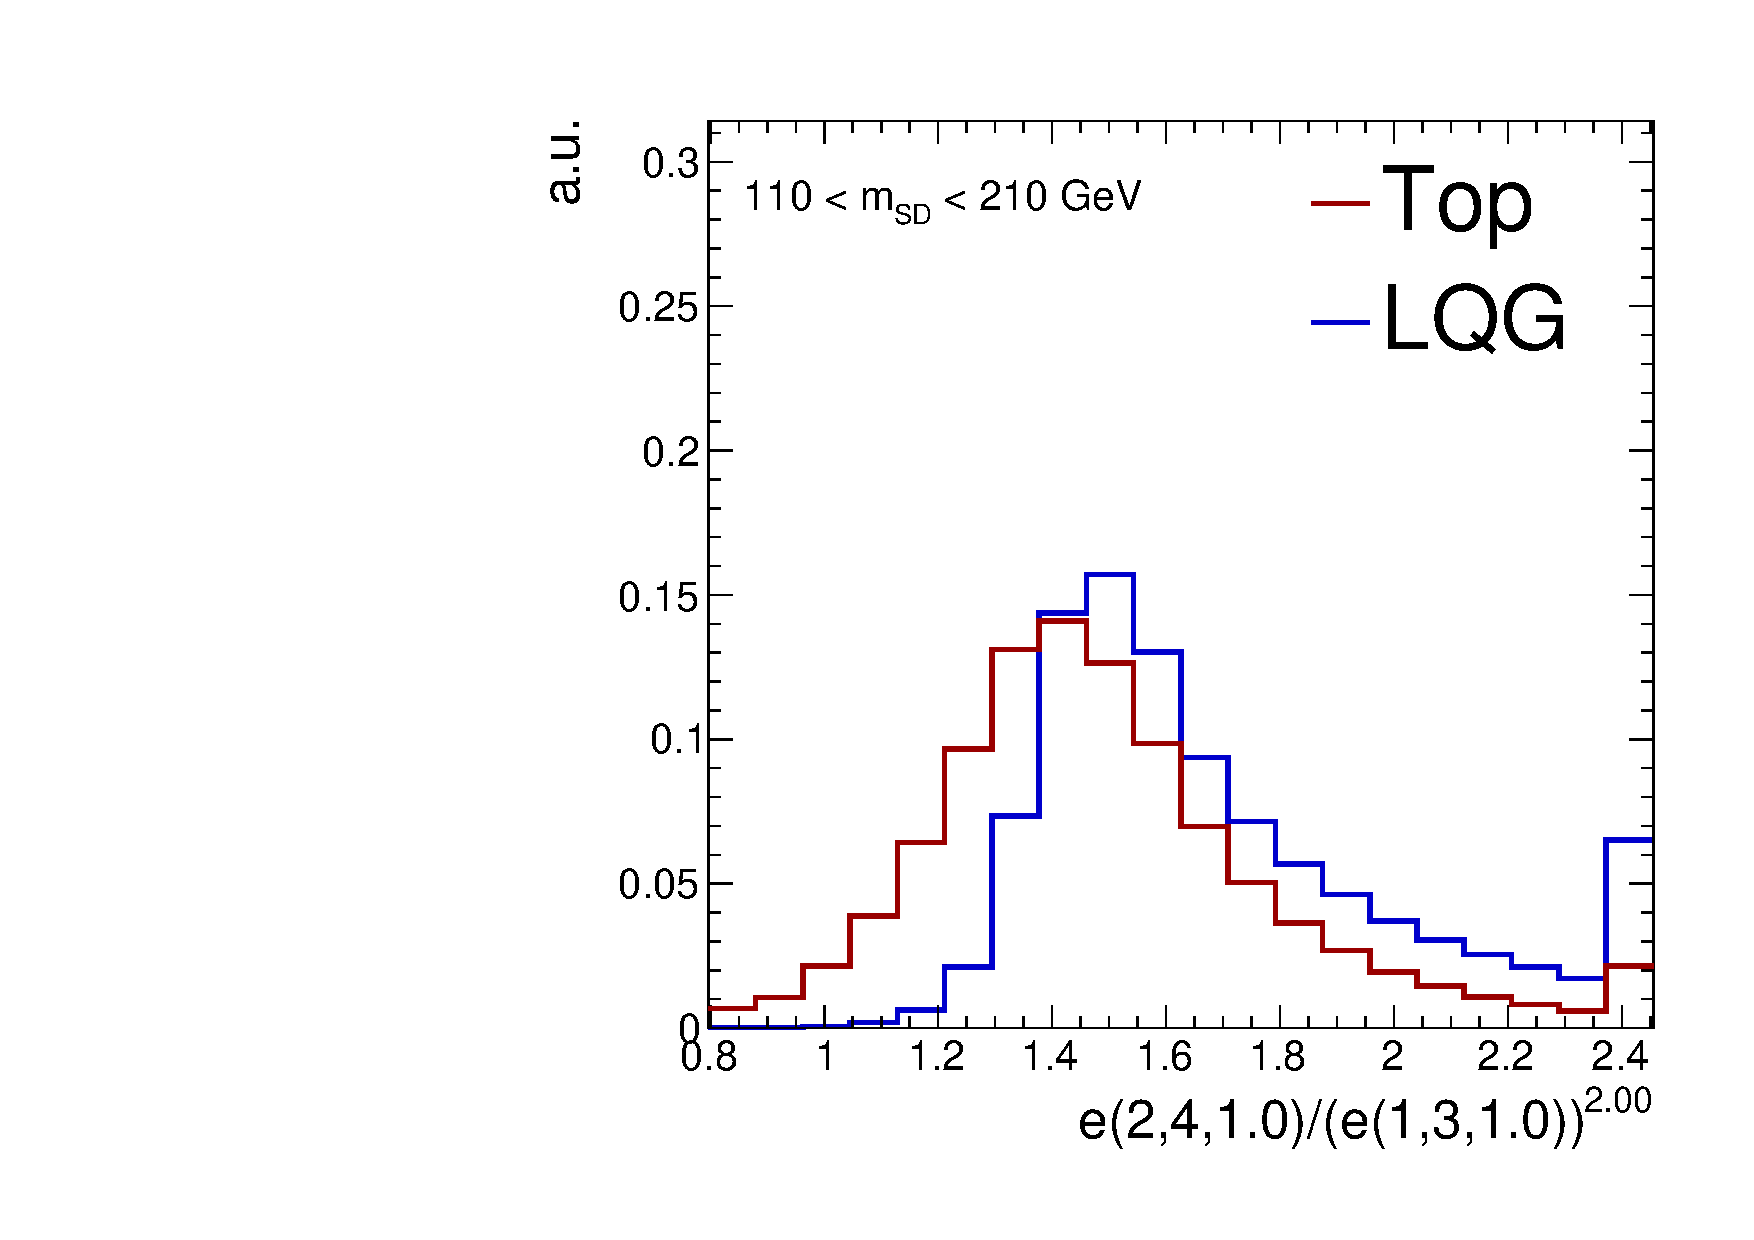
\includegraphics[width=\textwidth]{figures/toptagging/shapes/mass_ratio_24101310.pdf}
        \end{subfigure}
        \begin{subfigure}[t]{0.32\textwidth}
            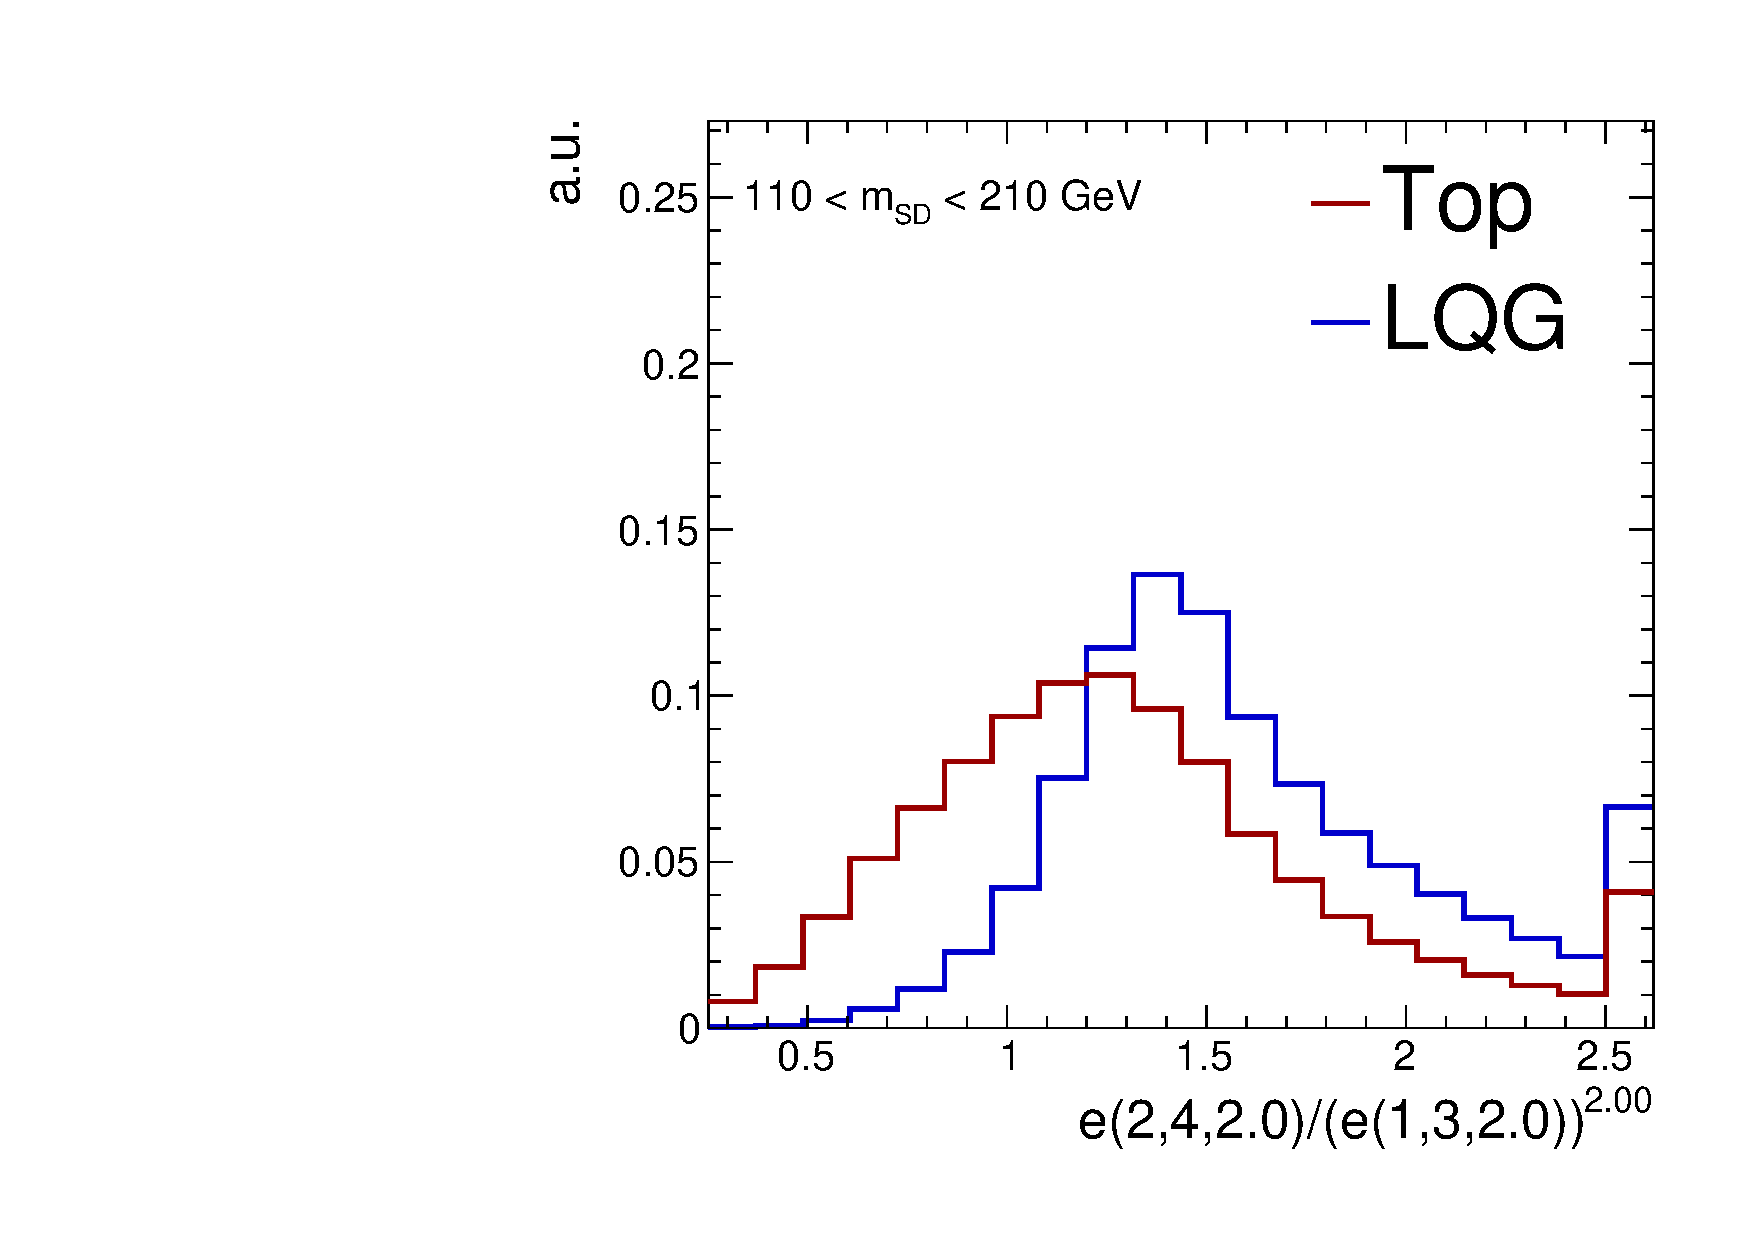
\includegraphics[width=\textwidth]{figures/toptagging/shapes/mass_ratio_24201320.pdf}
        \end{subfigure}
        \begin{subfigure}[t]{0.32\textwidth}
            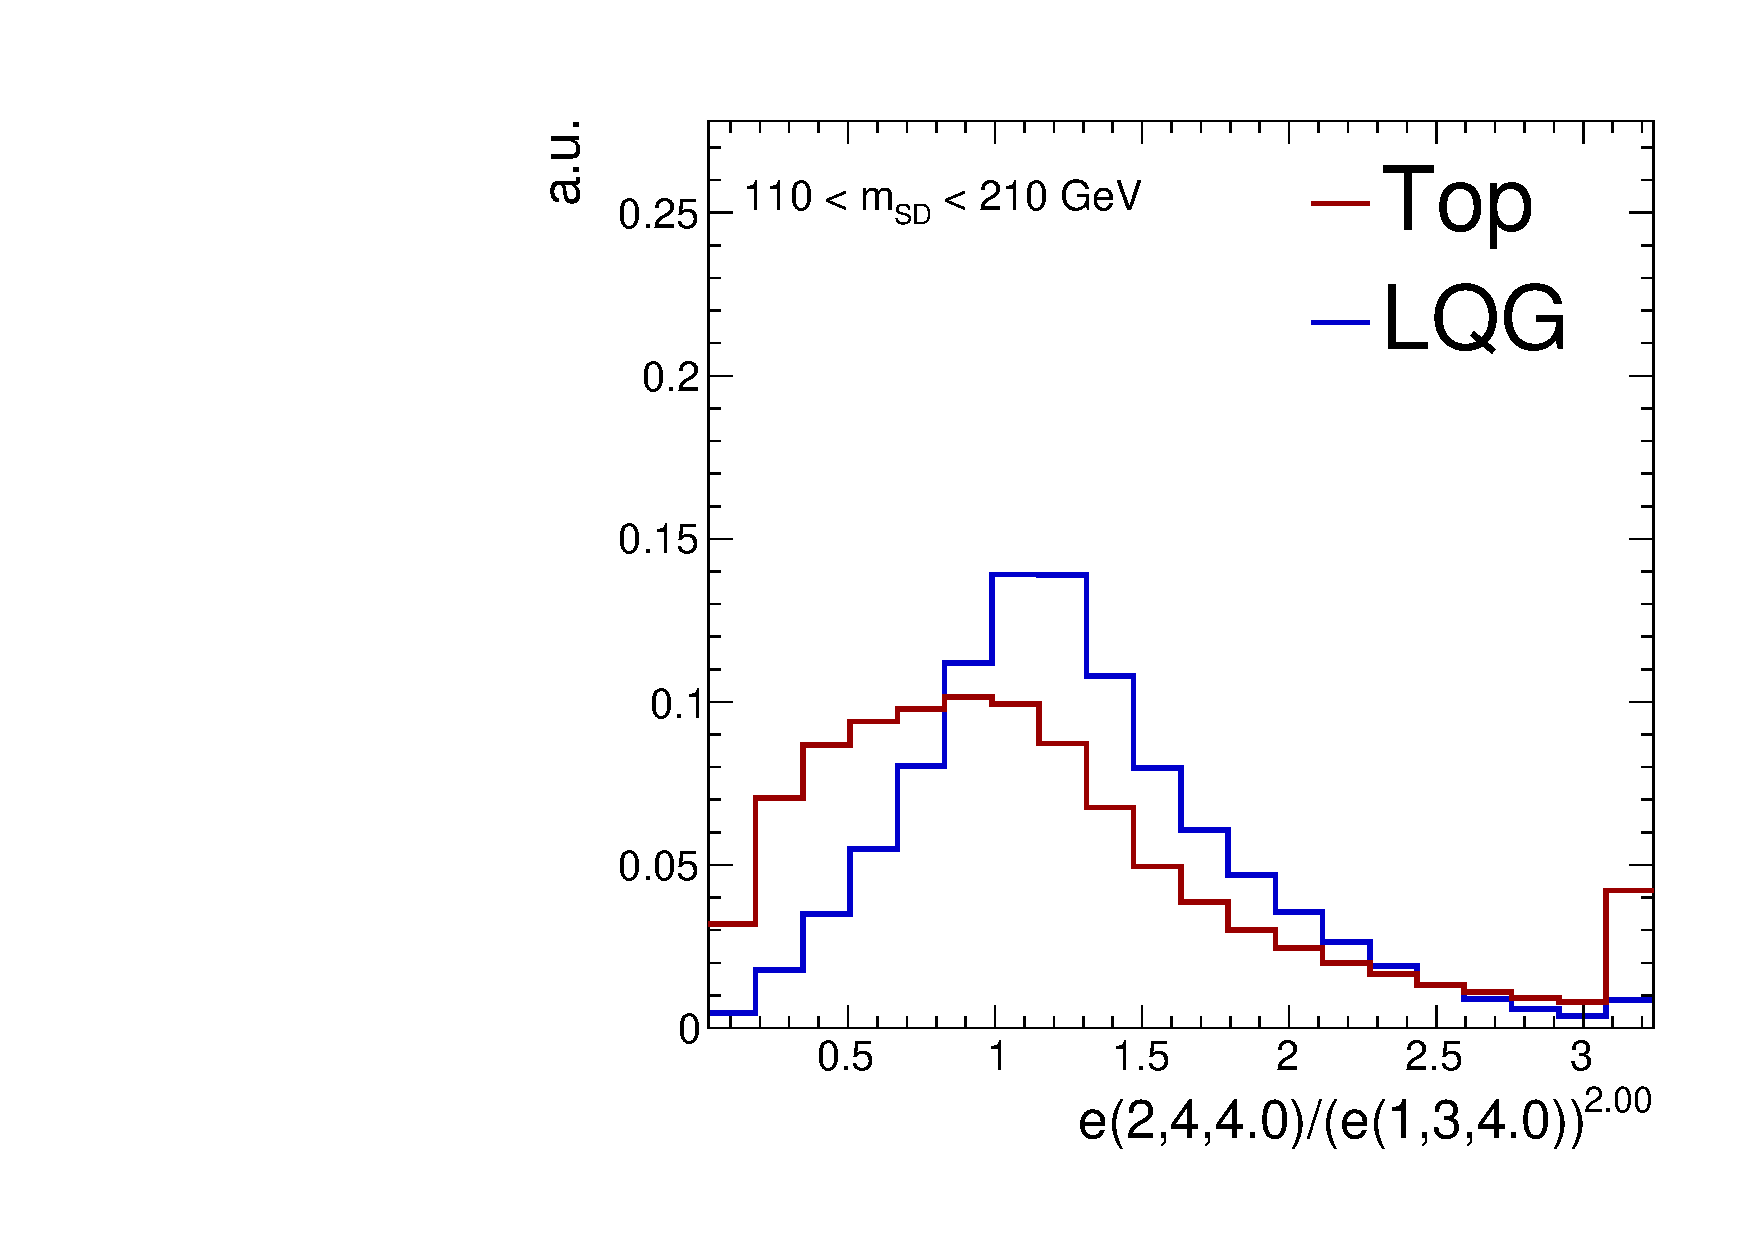
\includegraphics[width=\textwidth]{figures/toptagging/shapes/mass_ratio_24401340.pdf}
        \end{subfigure}
        \caption{Shape of the $N_3$ observables in top and LQG jets, for various values of $\beta$.}
        \label{fig:jets:n3}
    \end{center}
\end{figure}

While $N_3$ has a strong theoretical motivation, it is possible that other functions of ECFs  distinguish between top and LQG jets.
In order to construct observables that do not have a strong dependence on the jet \pt, we restrict ourselves to ratios of the form:
\begin{equation}
    \psi(a,N,\alpha,b,M,\beta) = 
    \frac{e(a,N,\alpha)}{\left(e(b,M,\beta)\right)^x} 
    \text{, where } M\leq N \text{ and } x = \frac{a\alpha}{b\beta}
\end{equation}
A large subset of this broader class of ECF observables are found to be useful (Figure~\ref{fig:jets:ecfrs}), including ratios not of the form $e(N=4)/e(N=3)$.

\begin{figure}[]
    \begin{center}
        \begin{subfigure}[t]{0.32\textwidth}
            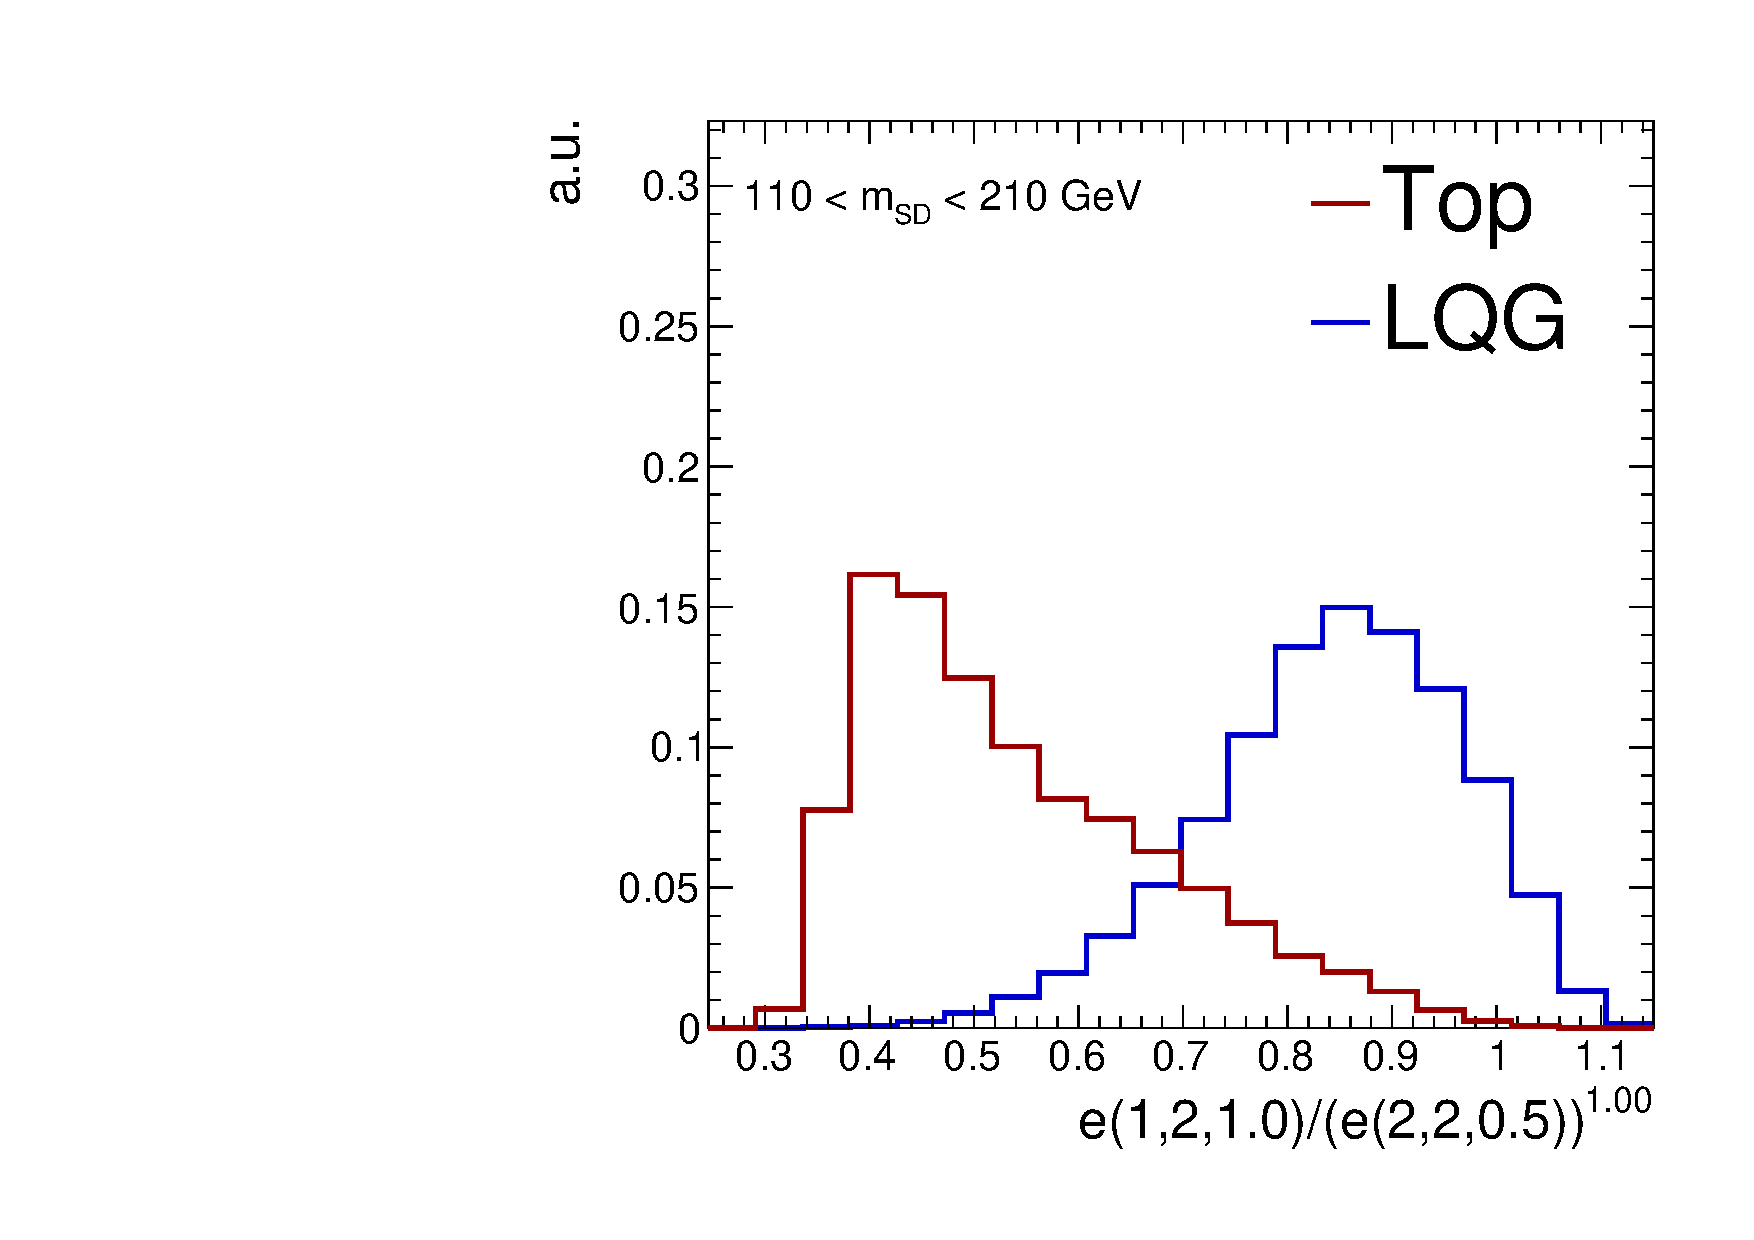
\includegraphics[width=\textwidth]{figures/toptagging/shapes/mass_ratio_12102205.pdf}
        \end{subfigure}
        \begin{subfigure}[t]{0.32\textwidth}
            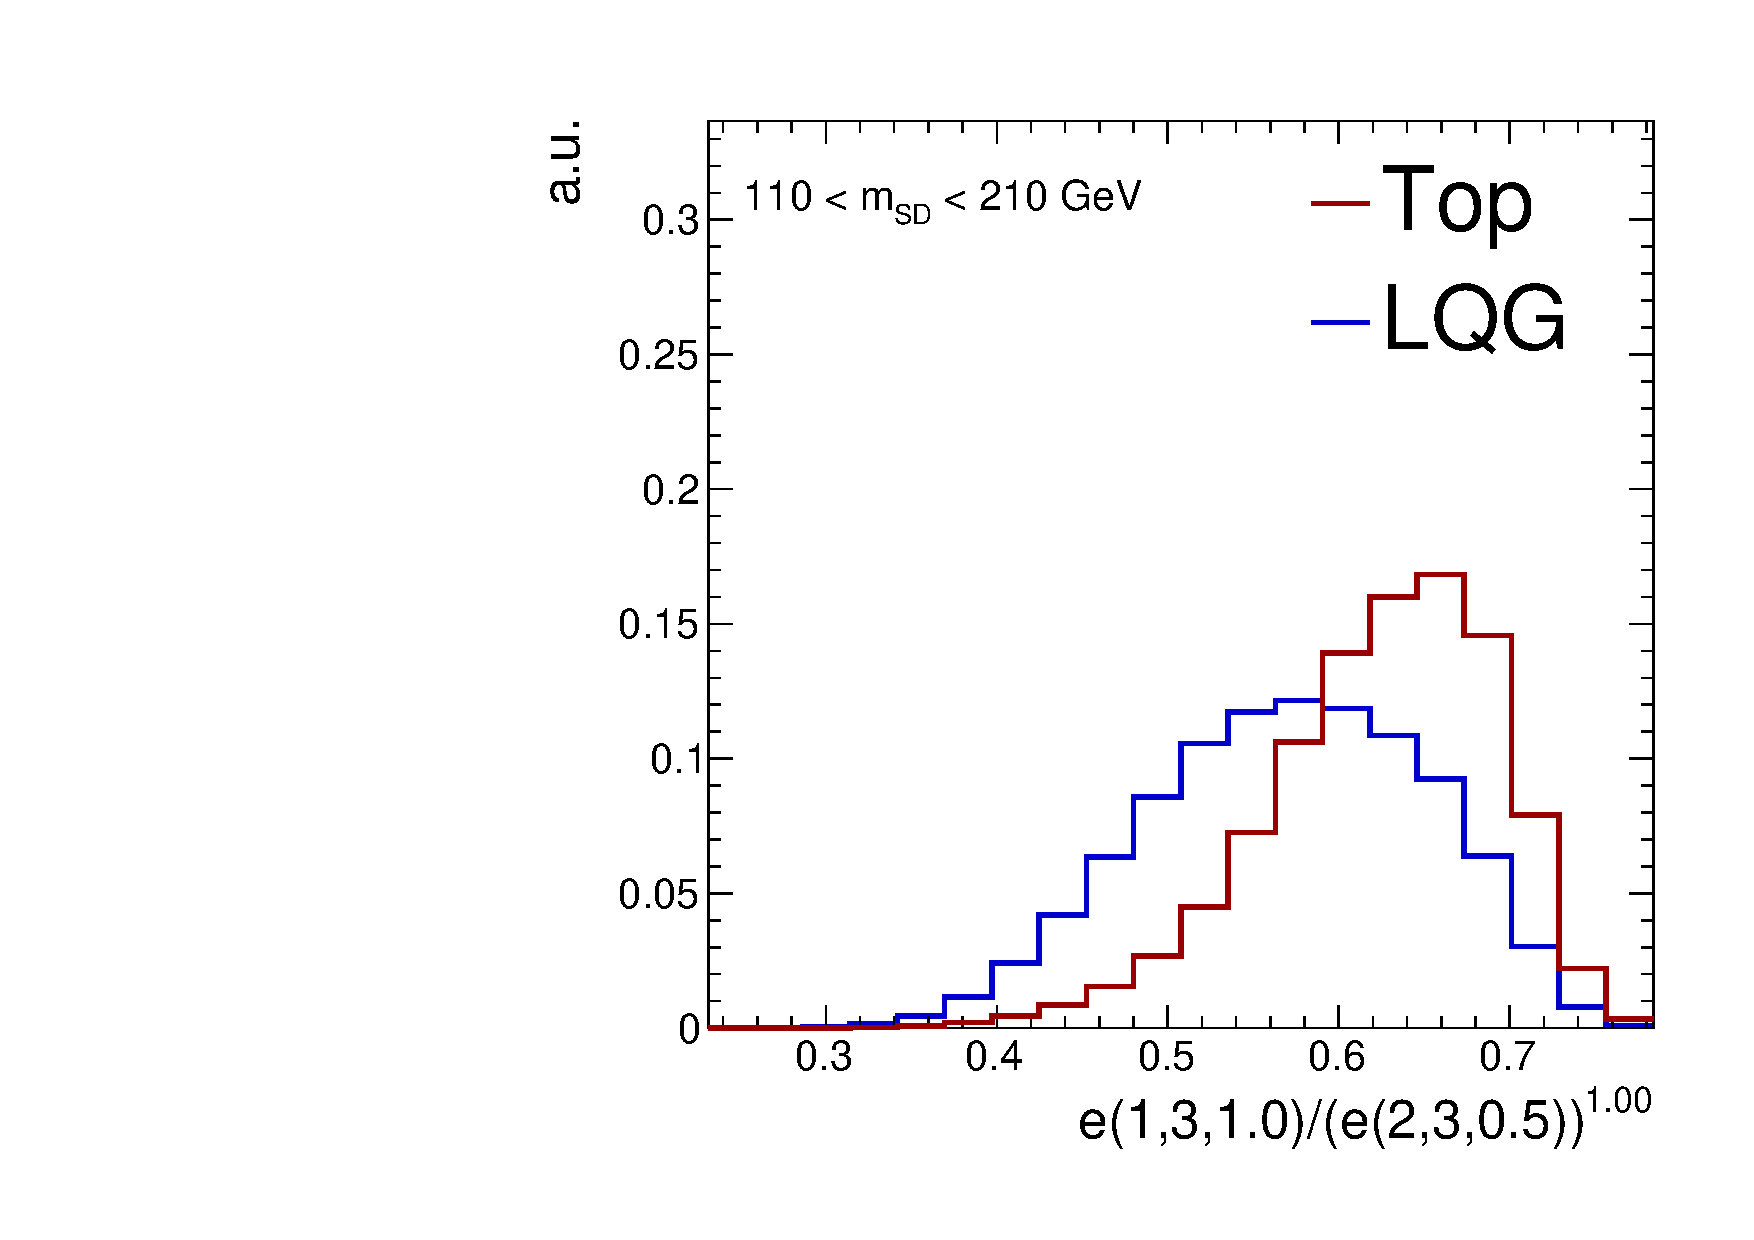
\includegraphics[width=\textwidth]{figures/toptagging/shapes/mass_ratio_13102305.pdf}
        \end{subfigure}
        \begin{subfigure}[t]{0.32\textwidth}
            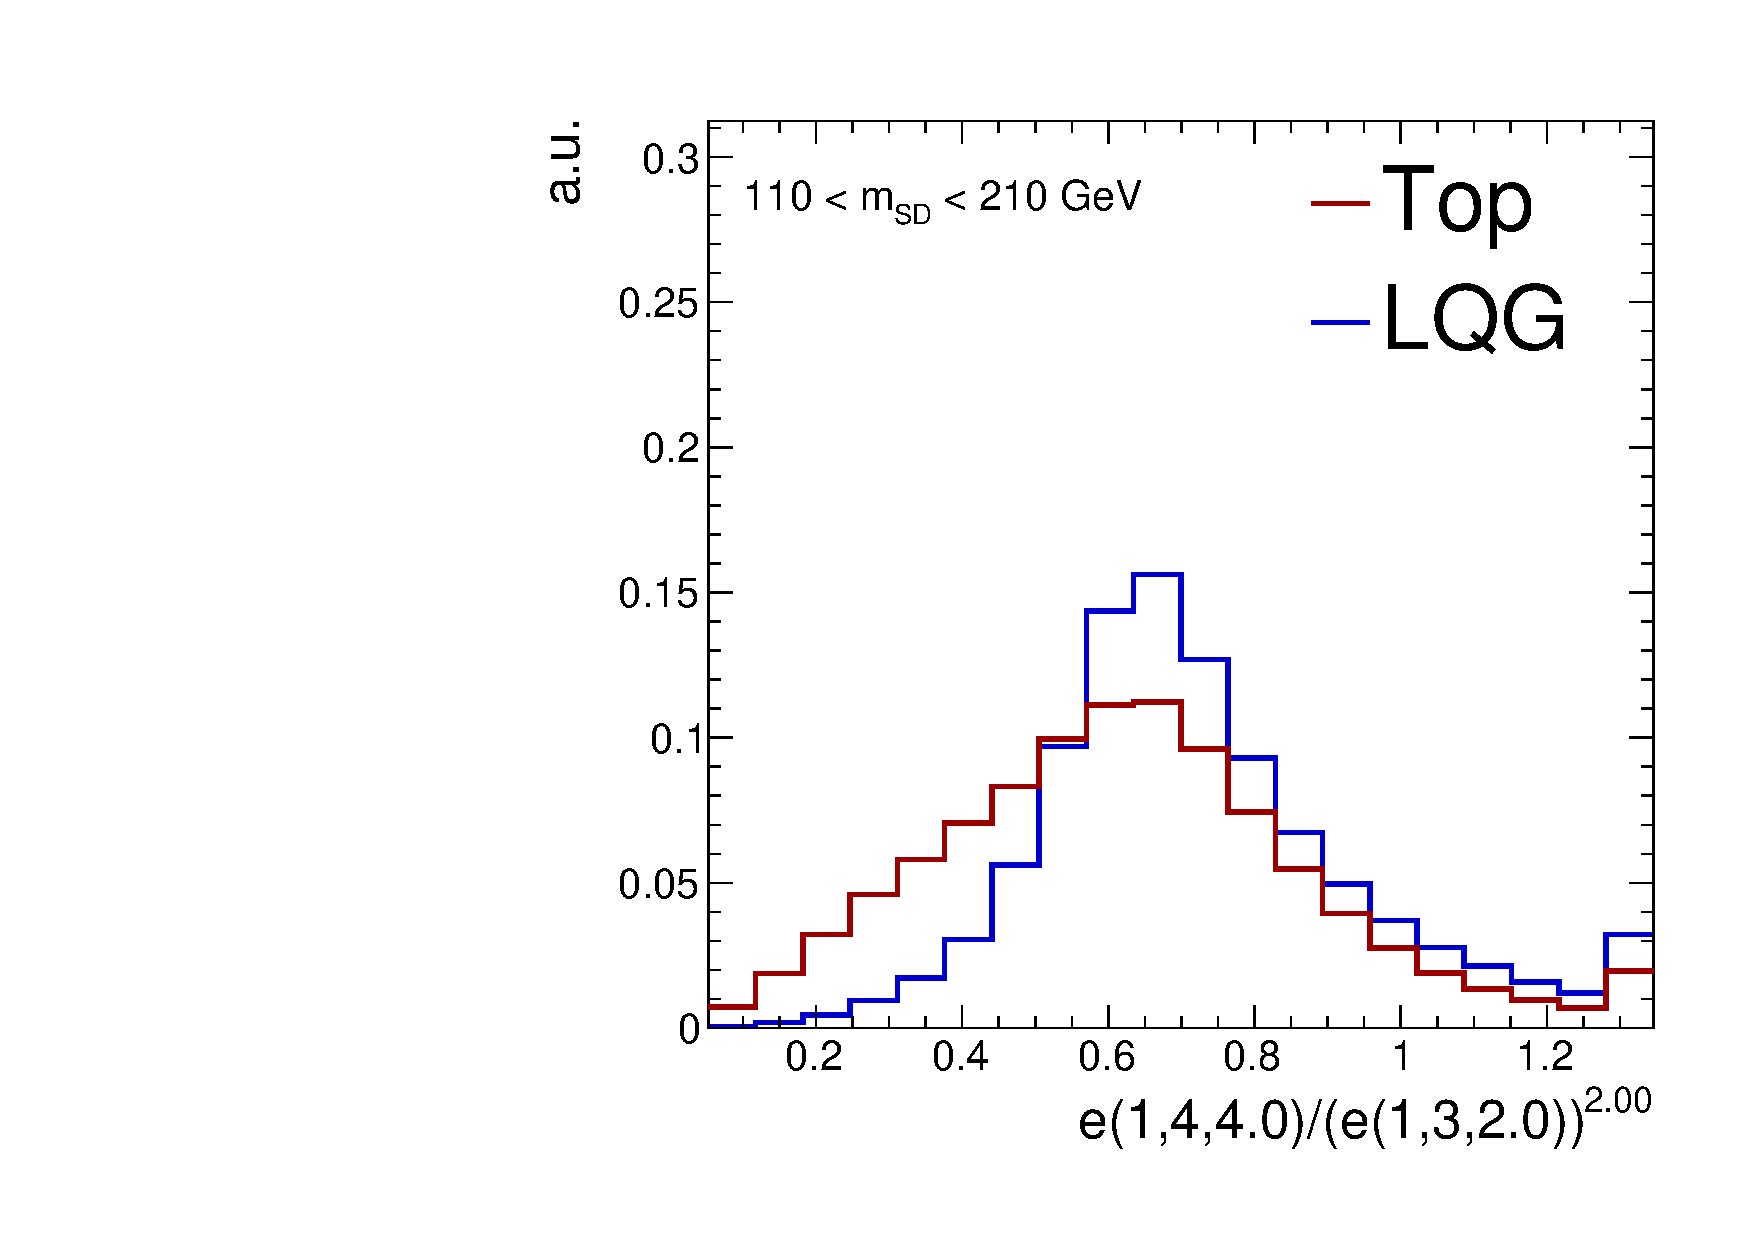
\includegraphics[width=\textwidth]{figures/toptagging/shapes/mass_ratio_14401320.pdf}
        \end{subfigure}
        \caption{Examples of non-trivial ECF ratios other than $N_3$ that separate top and LQG jet distributions.}
        \label{fig:jets:ecfrs}
    \end{center}
\end{figure}


\subsection{A combined tagger}
\label{sec:jets:bdt}

In principle, we have constructed an infinitely large space of substructure observables.
In practice, we only consider a finite sampling of ECF parameters:
\begin{gather}
    N \in \{1,2,3,4\} \nonumber \\ 
    o \in \{1,2,3\} \nonumber \\ 
    \beta \in \{0.5, 1, 2, 4\}
\end{gather}
This grid results in $\sim900$ $\psi$ observables.

To build a single optimal observable out of all the $\{\psi_i\}$s, we will use a boosted decision tree (BDT).
A simplified algorithm to train a single decision tree node $n$ is as follows:
\begin{enumerate}
    \item Choose a $\psi_j$, either by sampling randomly or selecting the one most optimal for the next step.
    \item Based on the training data fed to the node, select a decision boundary $d_n$ to optimize a loss function. For example, one can use the cross-entropy loss:
        \begin{gather}
            \ell(X,y;j,d_n) =  -\hat\pi_B\ln\hat\pi_B -\hat\pi_S\ln\hat\pi_S \text{, where } 
            \hat\pi_c = \hat P(y=c | \psi_j < d_n) 
        \end{gather}
\end{enumerate}
A tree is built iteratively:
\begin{enumerate}
    \item Train a node $n$ using the above criteria. 
    \item If a stopping condition is not met (i.e. maximum number of nodes, minimal improvement in $\ell(n)$), train one node on the samples that pass $n$ and another on the samples that fail.
\end{enumerate}
Figure~\ref{fig:jets:dt} provides a pictoral example of how a decision tree can be built. 

\begin{figure}[]
    \begin{center}
        \begin{subfigure}[t]{0.32\textwidth}
            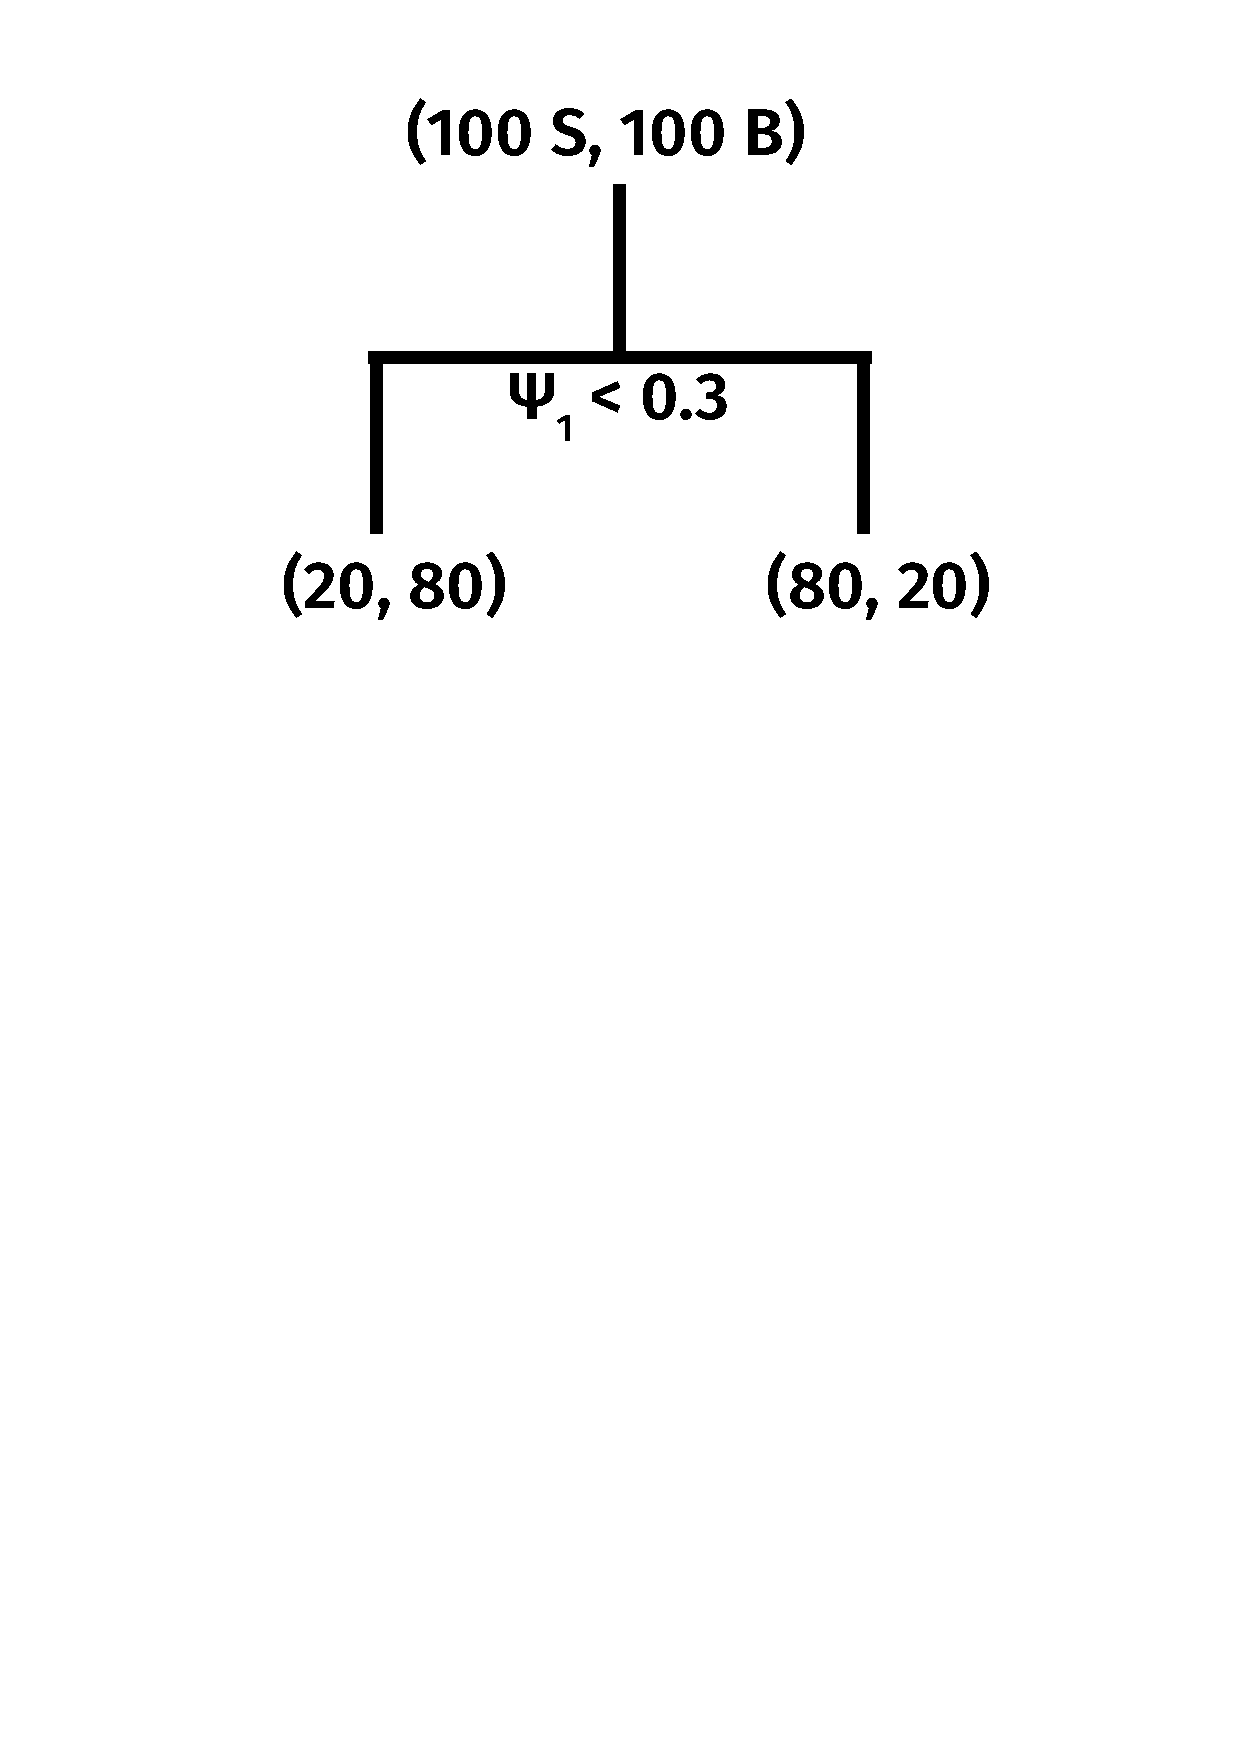
\includegraphics[width=\textwidth]{figures/toptagging/bdt/tree0.pdf}
        \end{subfigure}
        \begin{subfigure}[t]{0.32\textwidth}
            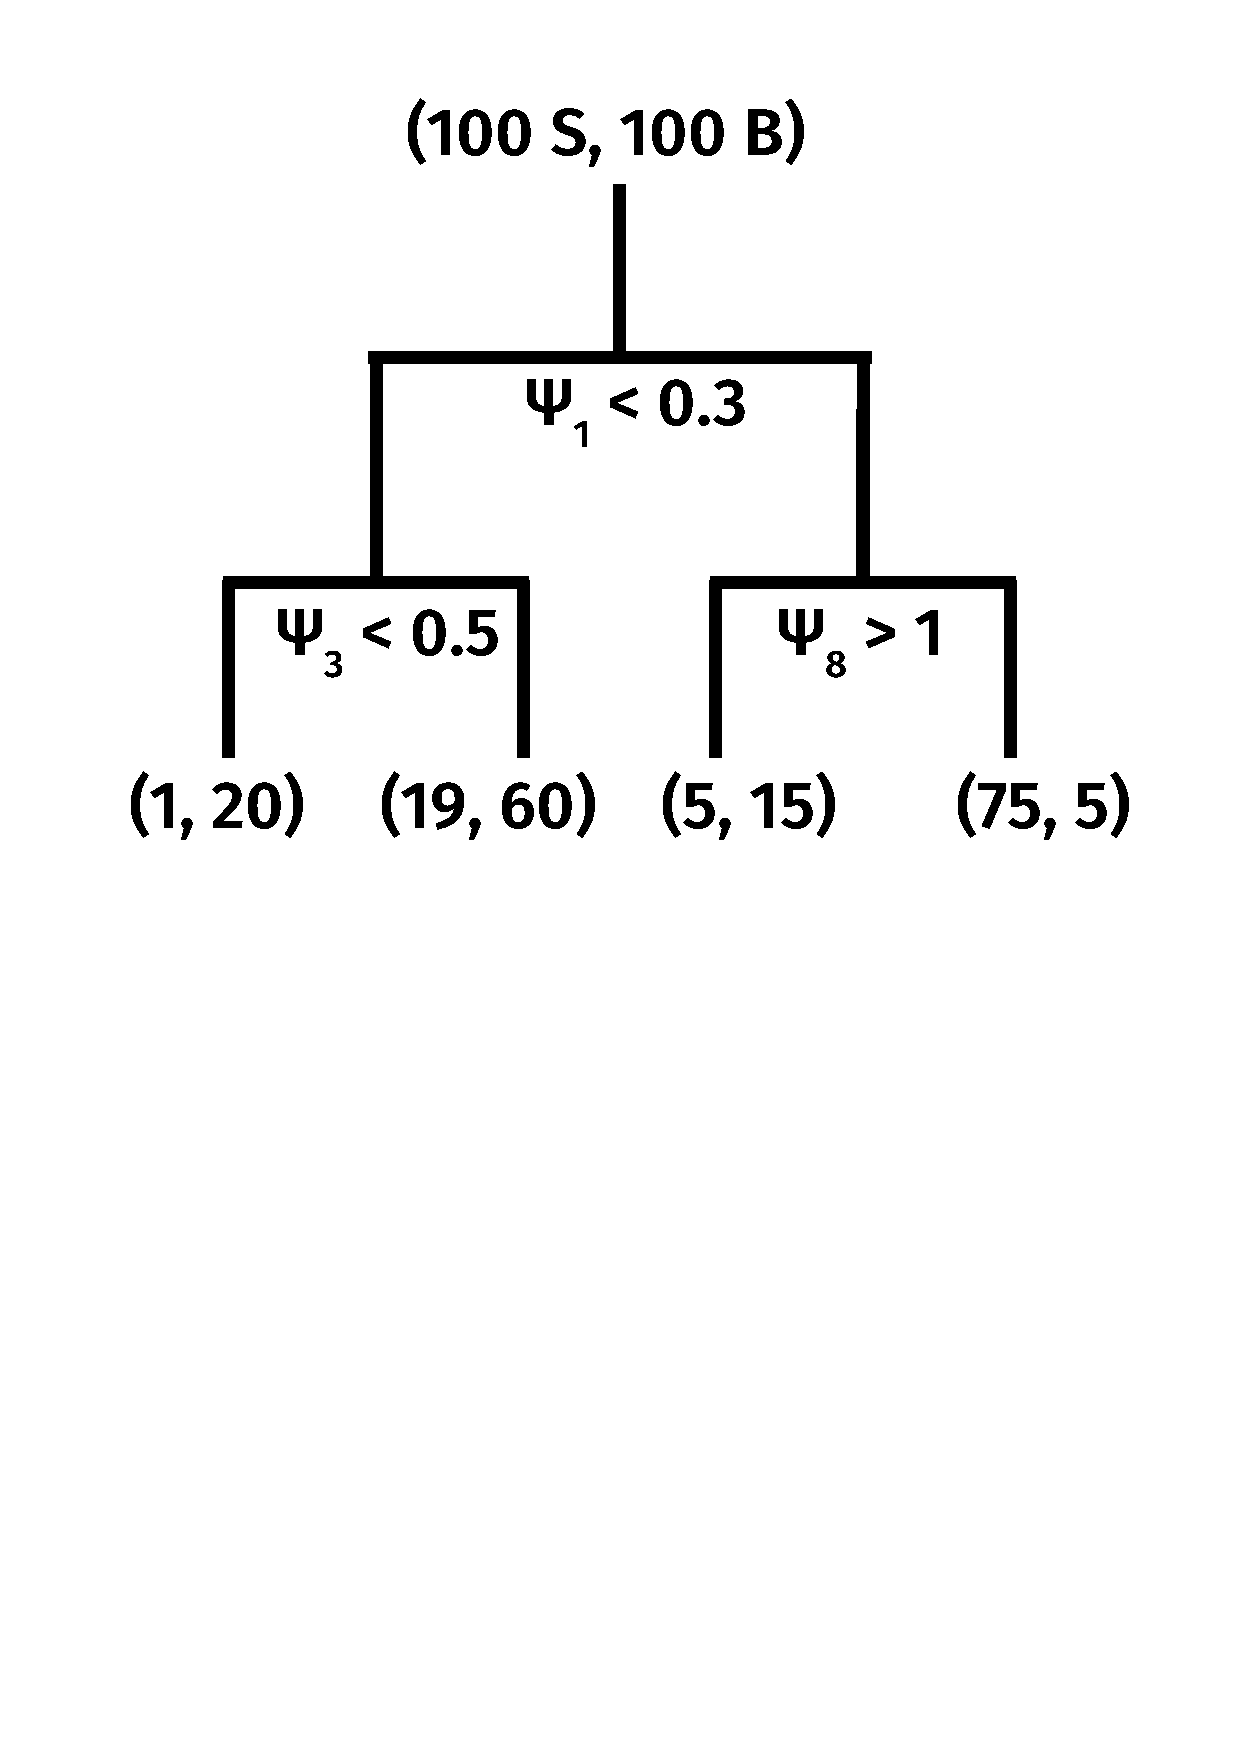
\includegraphics[width=\textwidth]{figures/toptagging/bdt/tree1.pdf}
        \end{subfigure}
        \begin{subfigure}[t]{0.32\textwidth}
            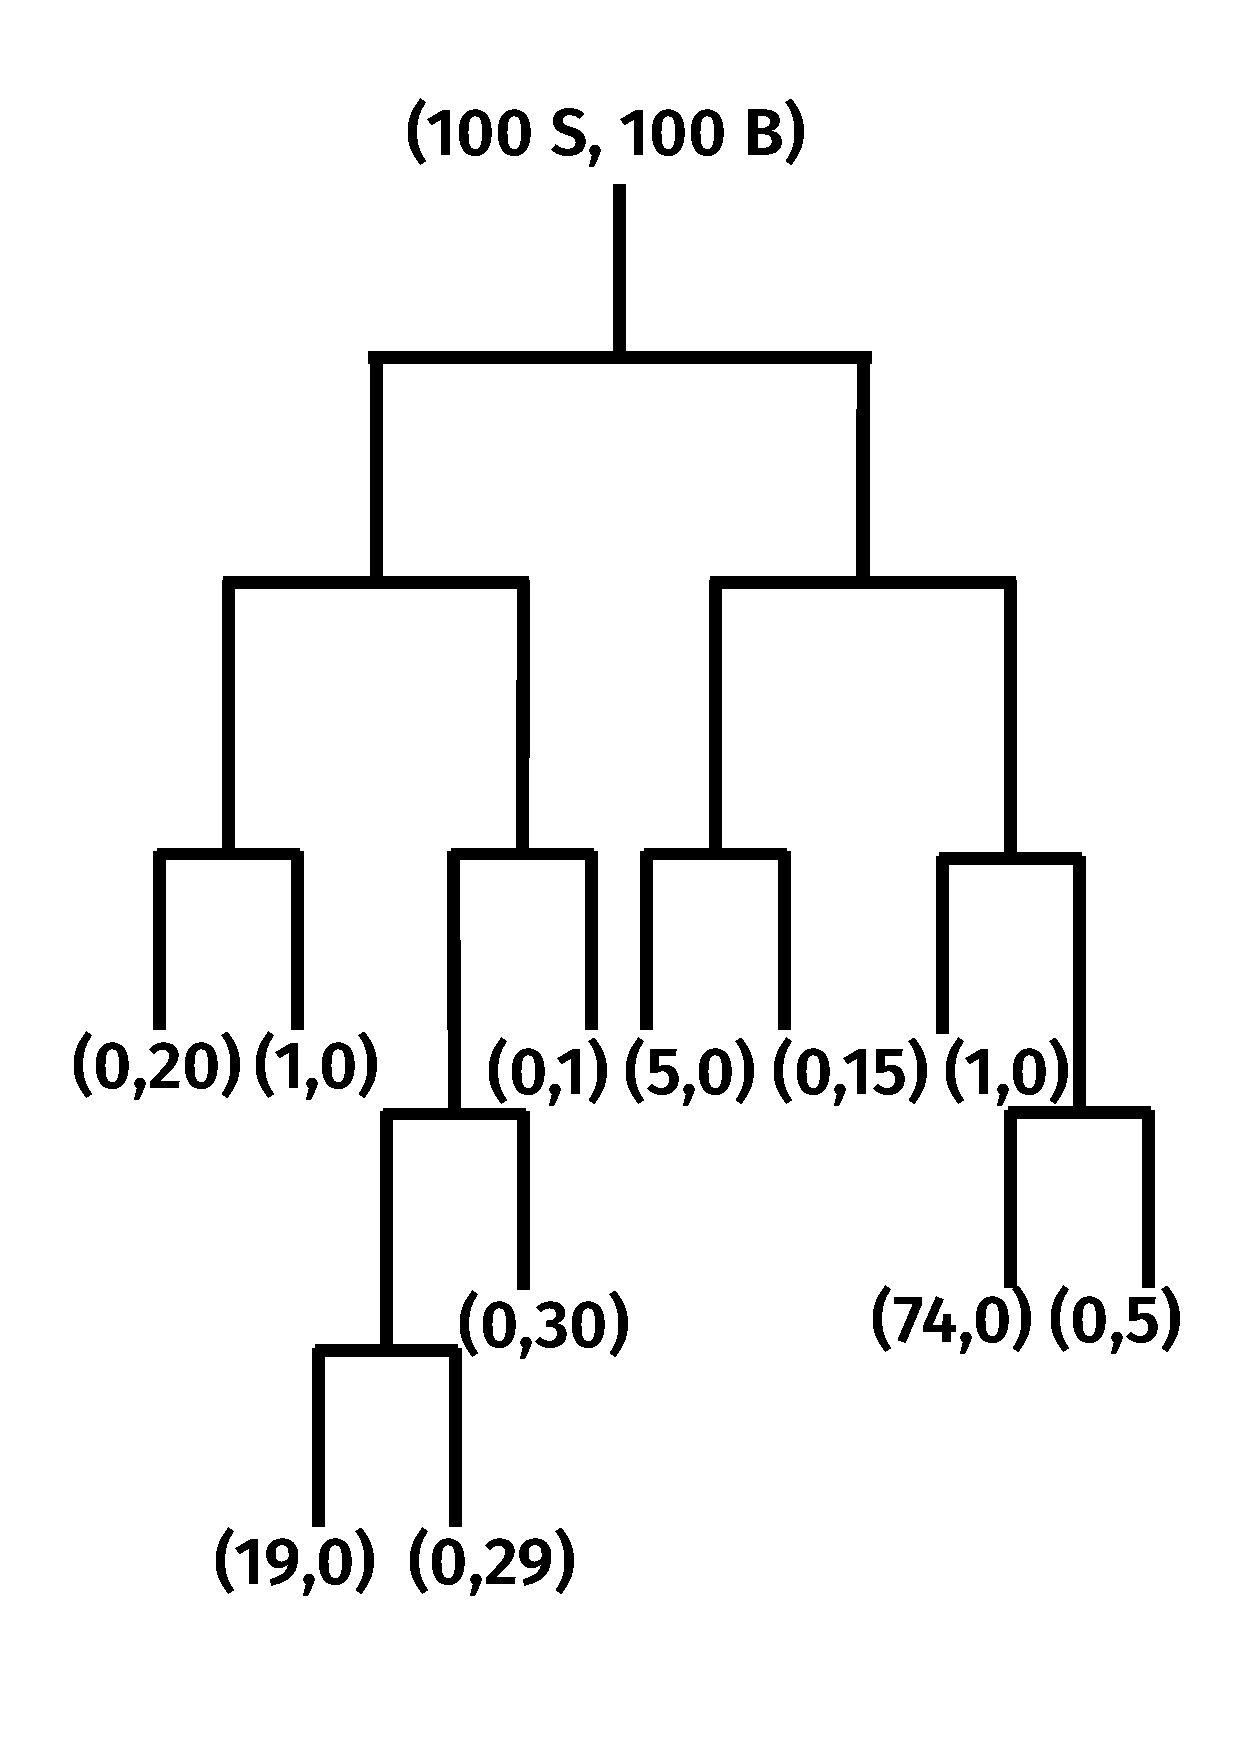
\includegraphics[width=\textwidth]{figures/toptagging/bdt/tree2.pdf}
        \end{subfigure}
        \caption{Steps in greedily training a simple decision tree.}
        \label{fig:jets:dt}
    \end{center}
\end{figure}

While decision trees can very accurately describe training data provided sufficient complexity, they also pathologically overfit the data.
To mitigate this, while retaining descriptive power, a standard method is to \emph{boost} many simple trees.
The simplicity of the tree prevents overfitting, while boosting many trees allows for a complex model.
The result of a BDT is a classifier $f_n(x) = \sum_{i=0}^n \nu^i T_i(x)$, where $\nu\leq 1$ is tunable and each $T_i$ is a decision tree. 
A simplified algorithm to train a BDT is as follows:
\begin{enumerate}
    \item Define a global loss function, e.g.:
        \begin{equation} L(y_i; f_i) = \ln\left(1 + \exp(-y_if_i)\right)\end{equation}
    \item Train a single tree $T_0$ and initialize classifier $f_0 = T_0$
    \item Until some stopping condition (index $m=1,\dots$):
    \begin{enumerate}
      \item[3.1.] Compute the ``residual''
        \begin{equation}r_{mi} = -\nabla_f L(y_i; f) |_{f=f_{m-1}(\bm\psi_i)}\end{equation}
        \begin{equation}L = (y-f_m(\bm\psi))^2 \Rightarrow r_m = y - f_m(\bm\psi) \end{equation}
      \item[3.2.] Fit a regression tree $T_m$ to predict $r_{mi}$ as a function of $x_i$:
        \begin{equation}\ell(X,r_m;j,d,\hat{r}) = \sum_{i | \psi_{ji} < d} (r_{mi} - \hat r)^2\end{equation}
      \item[3.3.] Update $f_m = f_{m-1} + \nu T_m$
    \end{enumerate}
\end{enumerate}

While we would like to train a BDT on the entire space of $\{\psi\}$, there are two issues to be solved: poorly modeled ratios and a large feature space.
Firstly, not every ECF ratio is well-simulated by our MC (Figure~\ref{fig:jets:datamc_ratios}).
More systematically, we can compute the CDFs of each $\psi$ and define a score: 
\begin{equation}
    -\log_{10} \mathrm{KS}(F(\psi_i | \mathrm{data}), F(\psi_i | \mathrm{MC})) = -\log_{10} \max \left|F(\psi_i | \mathrm{data}) - F(\psi_i | \mathrm{MC})\right|
\end{equation}
where $F$ represents the CDF and $\mathrm{KS}$ denotes the Kolmogorov-Smirnov metric on probability distributions.
The score is close to 0 for poorly-simulated distributions.
Figure~\ref{fig:jets:ks} parameterizes this as a function of $N/M$ (ratio of the number of particles) and $a\alpha/b\beta$ (ratio of the angular powers) and shows an interesting structure.
It is found that $3/2$ and $4/2$ ratios are uniformly poorly modeled, as are ratios with large $a\alpha/b\beta$. 
While this structure is interesting and suggestive, we do not yet understand its origin, and therefore do not use this parameterization to select ECF ratios.
Instead, we simply reject any ECF ratio for which $-\log_{10}\mathrm{KS} < 1$. 

\begin{figure}[]
    \begin{center}
        \begin{subfigure}[t]{0.32\textwidth}
            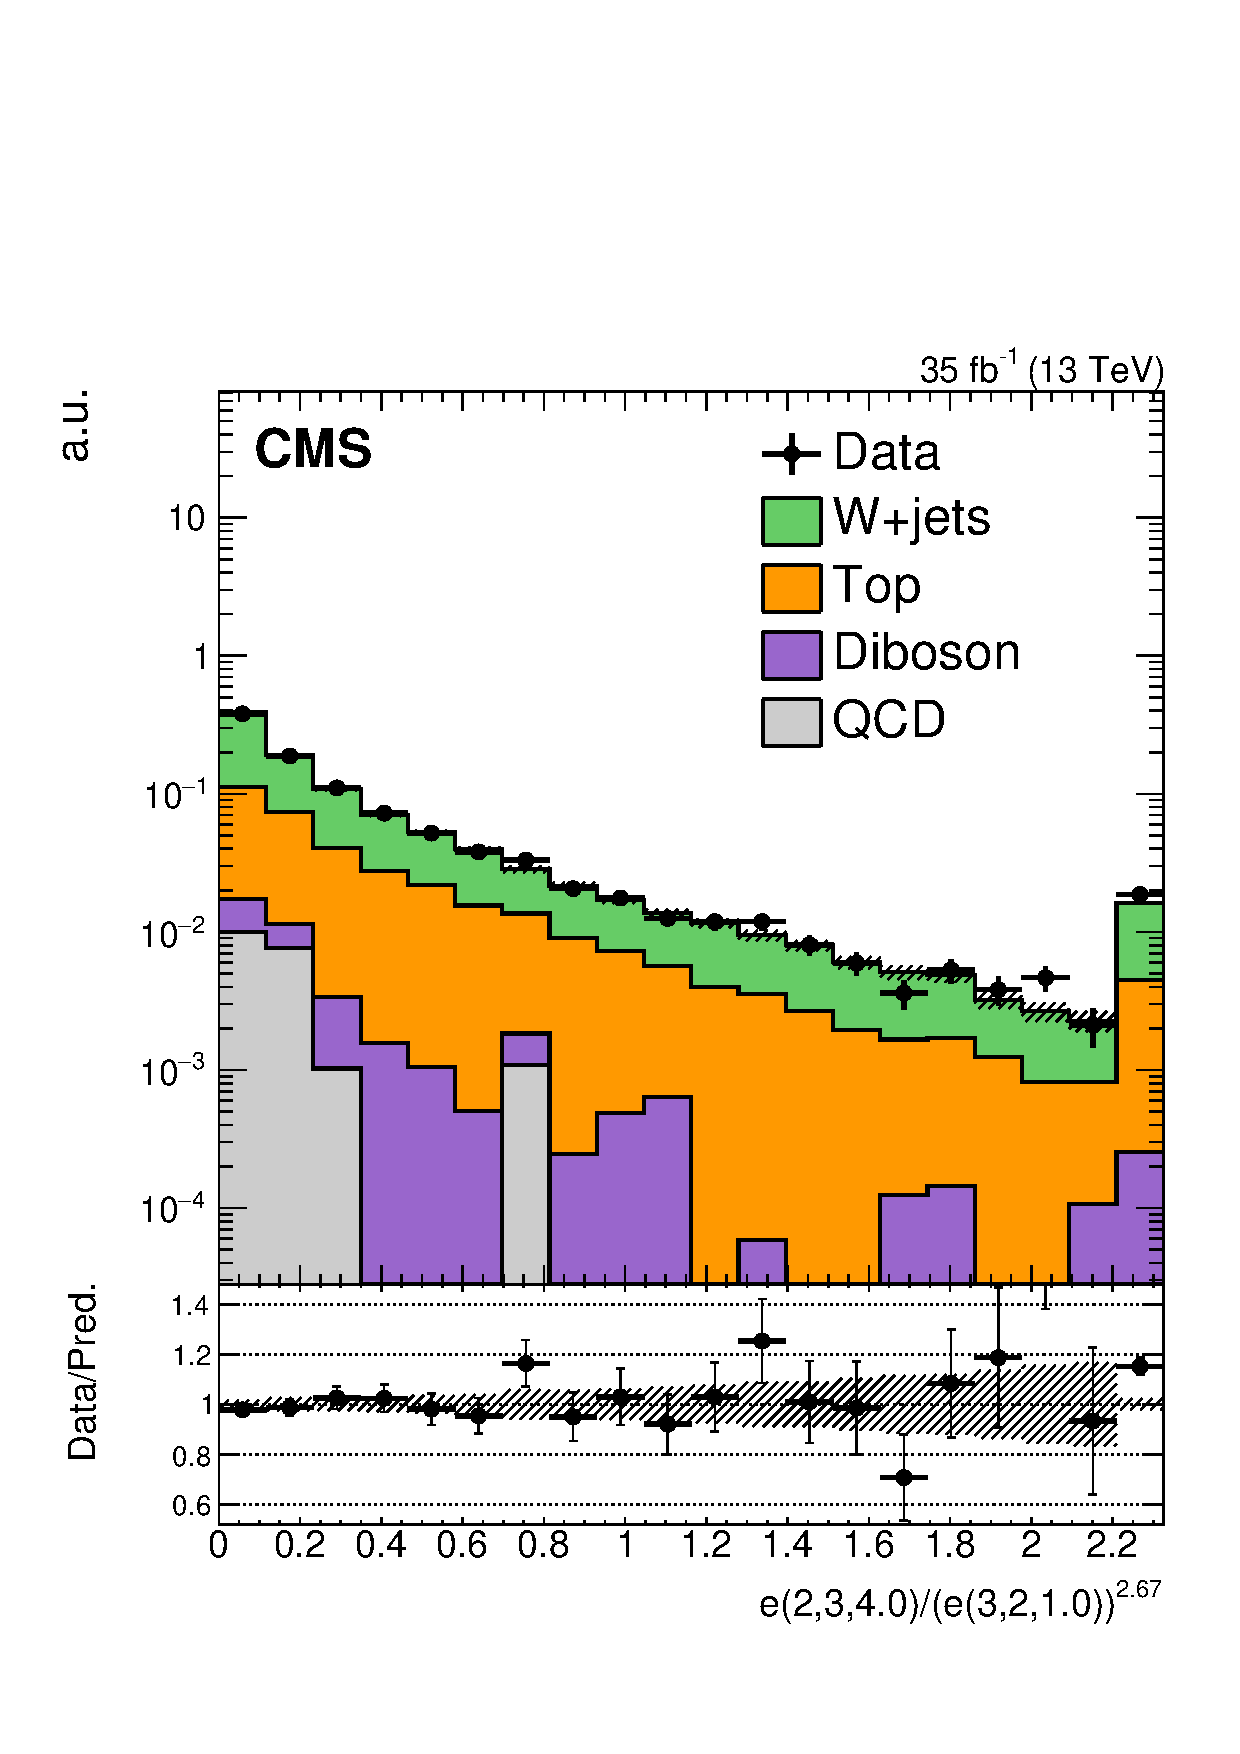
\includegraphics[width=\textwidth]{figures/toptagging/datamc/singlemuonw_ratio_23403210_logy.pdf}
        \end{subfigure}
        \begin{subfigure}[t]{0.32\textwidth}
            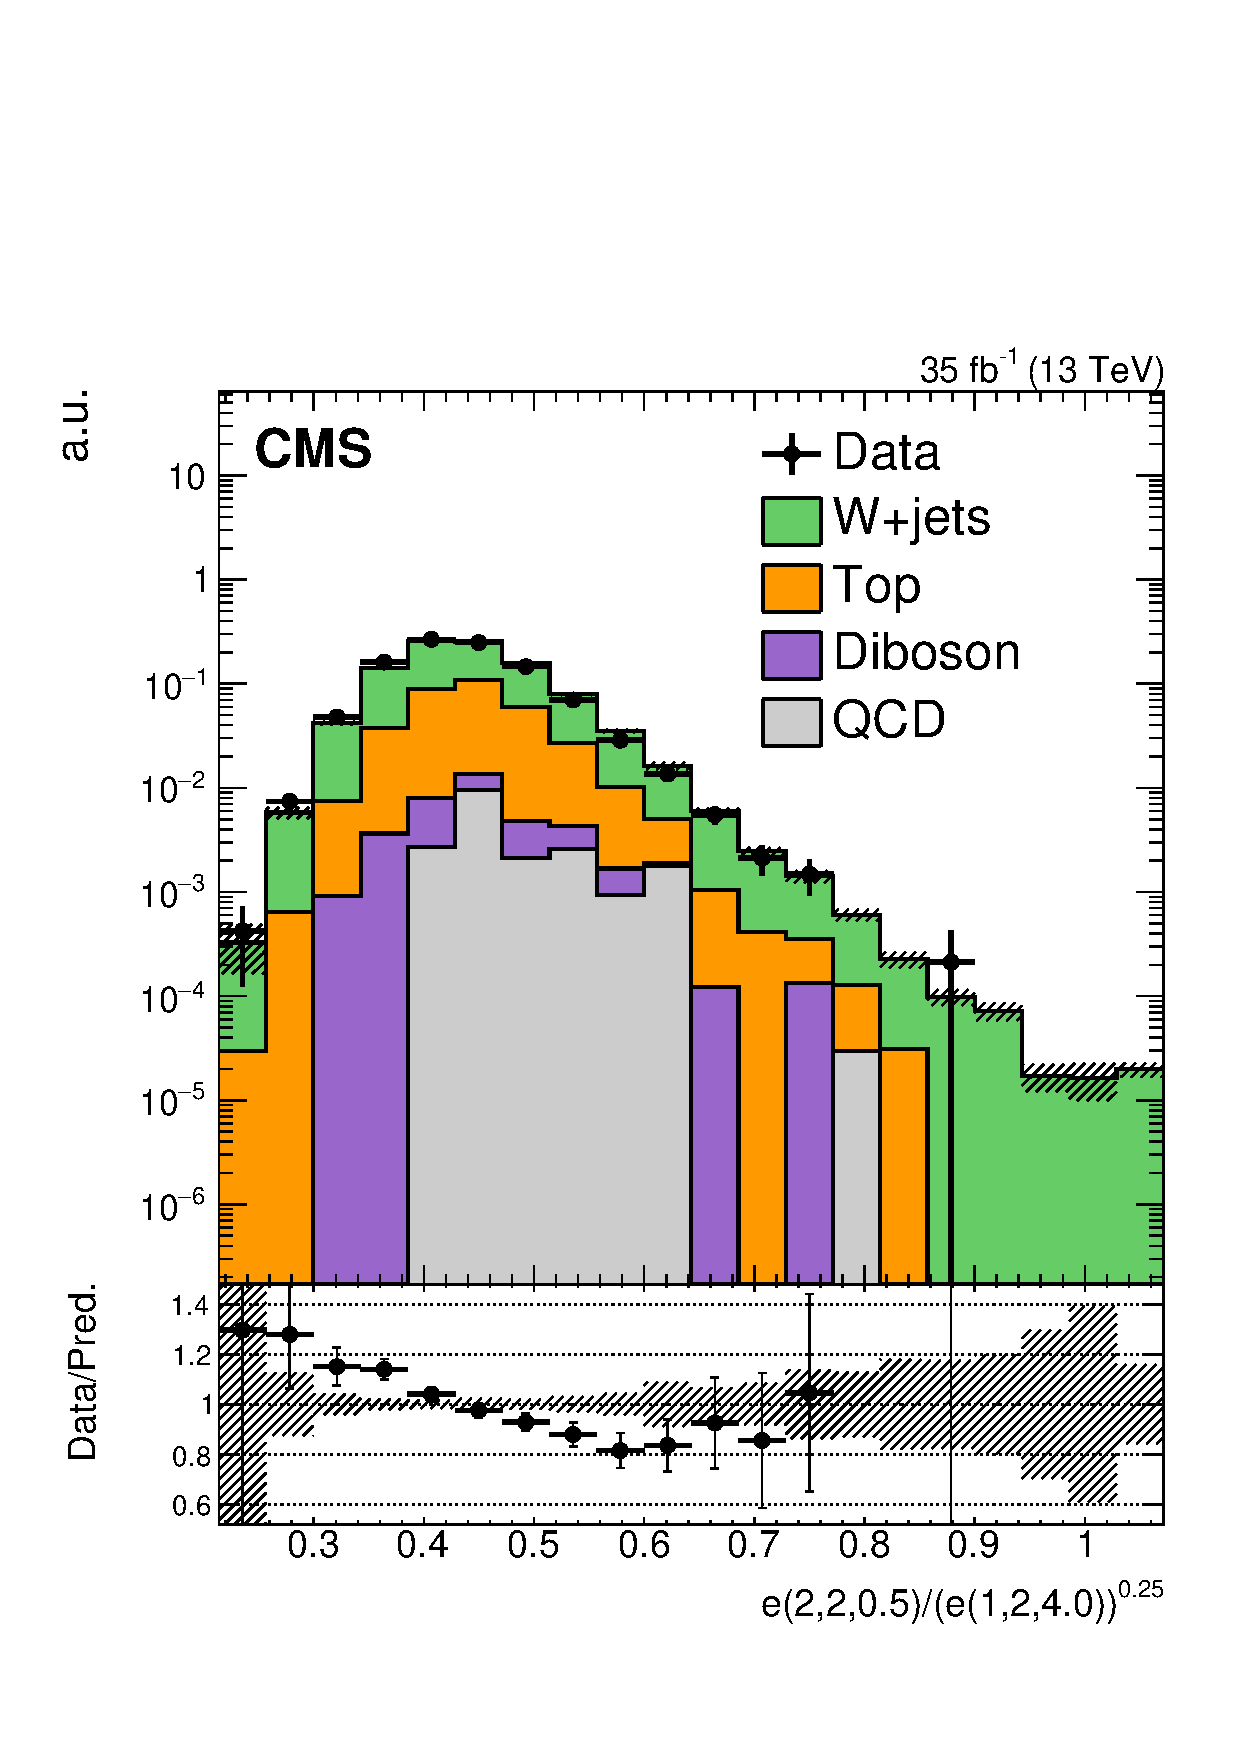
\includegraphics[width=\textwidth]{figures/toptagging/datamc/singlemuonw_ratio_22051240_logy.pdf}
        \end{subfigure}
        \caption{Two different ECF ratios in a $W$+jets selection, heavily enriched in LQG jets.
                 One is fairly well-modeled, while the other is not. }
        \label{fig:jets:datamc_ratios}
    \end{center}
\end{figure}

\begin{figure}[]
    \begin{center}
        \begin{subfigure}[t]{0.4\textwidth}
            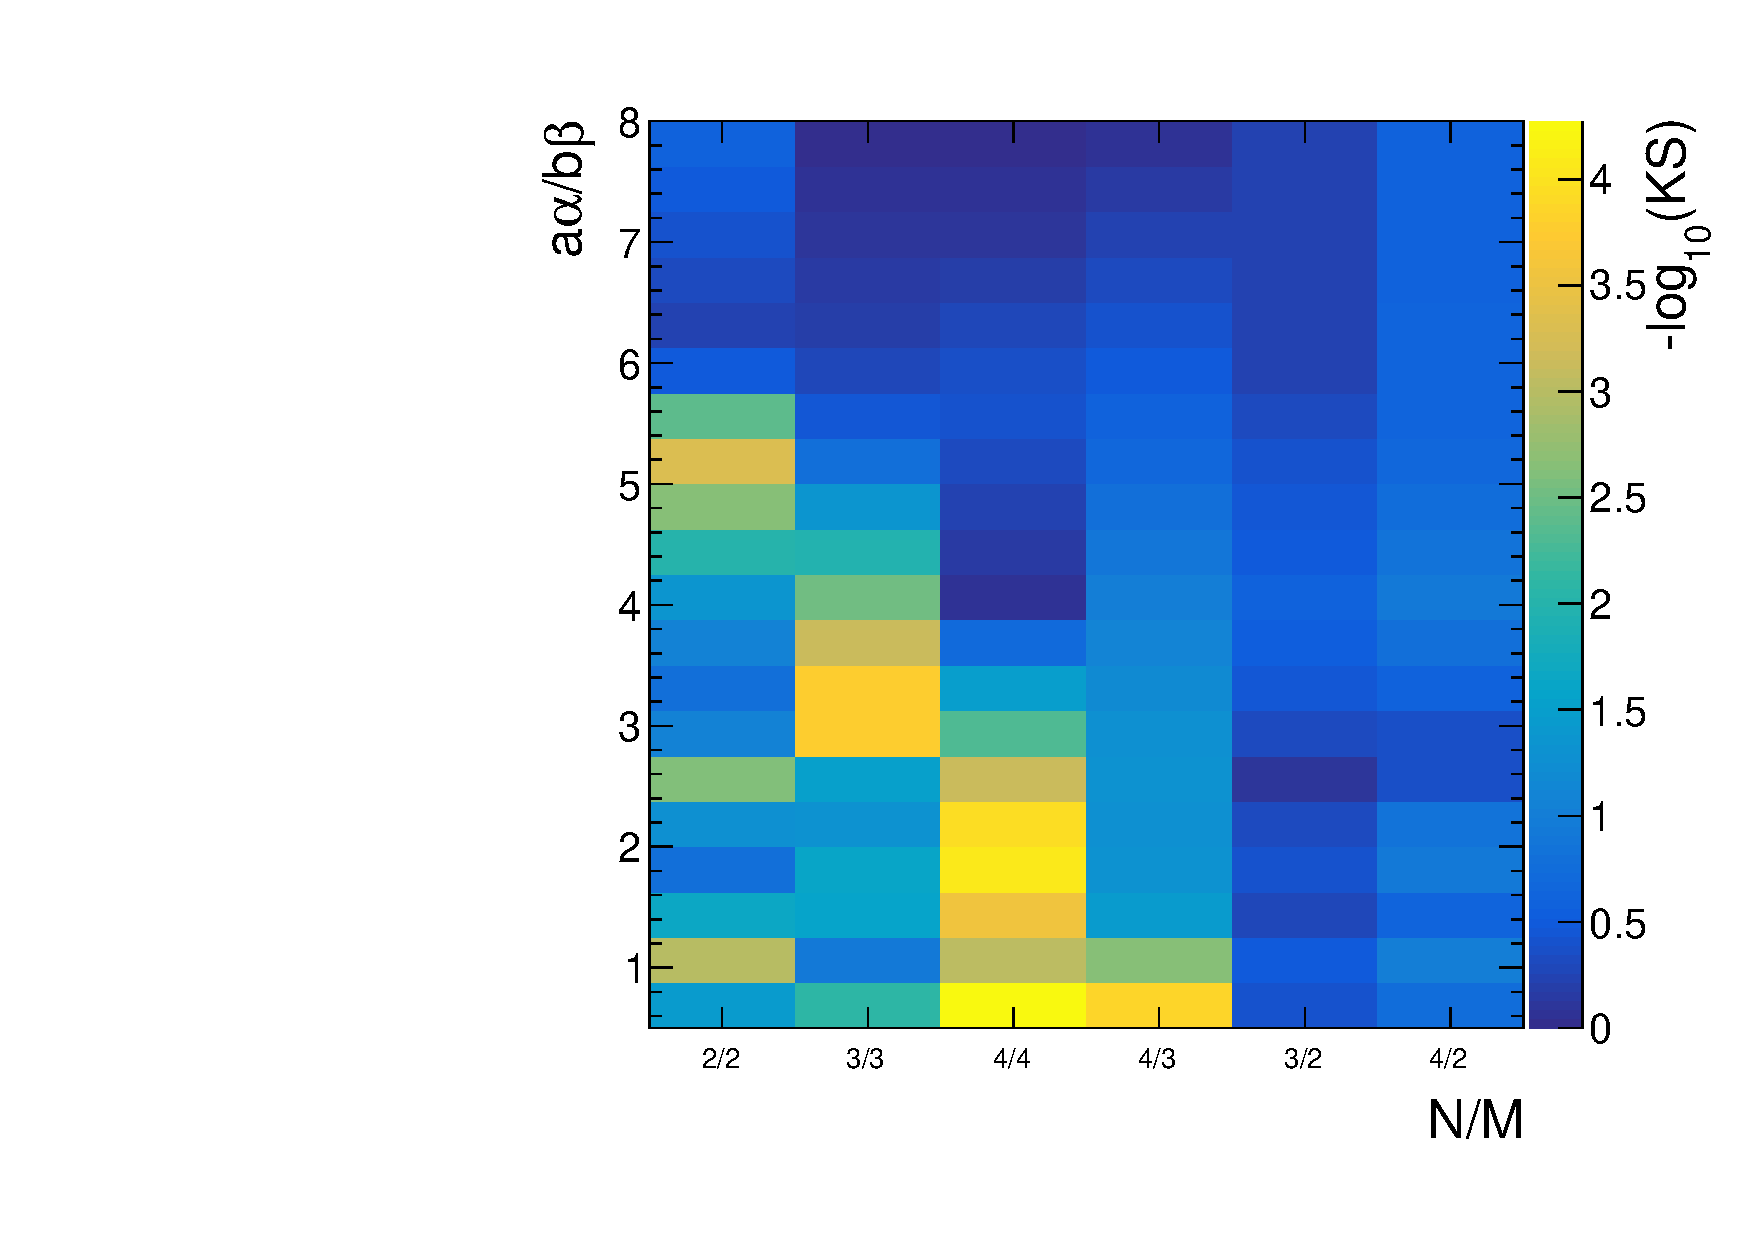
\includegraphics[width=\textwidth]{figures/toptagging/datamc/scanmnab.pdf}
        \end{subfigure}
        \caption{The $-\log_{10}\mathrm{KS}$ metric as a function of $N/M$ and $a\alpha/b\beta$, computed using events enriched in LQG jets. }
        \label{fig:jets:ks}
    \end{center}
\end{figure}

Even after filtering poorly-modeled ratios, we are left with a sampled $\psi$ grid of $\sim 400$ points.
By inspection, many of the $\psi$s are highly correlated or not useful at all.
It is desirable to reduce the size of the feature space, as computing each ECF is somewhat computationally-intensive: an $N$-point ECF on a $p$-particle jet has $\binom{N}{p}$ terms. 
Note that standard pre-processing techniques, like principal component analysis, do not reduce the number of features to be computed. 
While L1 regularization does attempt such a dimensional reduction, it cannot be trivially applied to BDTs. 
Therefore, we introduce a targeted iterative training method to solve this problem:
\begin{enumerate}
    \item Train a BDT with trees $T_1,\dots,T_n$
    \item For each $\psi_i$, define a score:
        \begin{equation}
             s_i = \sum_{m=1}^n \nu^{m-1} \sum_{\text{nodes using $\psi_i$ in $T_m$}} N_\text{samples}(\mathrm{node}) \times \left(\ell(\mathrm{node}) - \ell(\mathrm{parent})\right)^2  
        \end{equation}
    \item Remove (one or more) $\psi_i$ with smallest $s_i$ and repeat until the global loss $L$ worsens significantly
\end{enumerate}
Iterative training is expensive and can require the training of $\mathcal{O}(50)$ BDTs.
It is semi-parallelizable, and the entire process typically takes a few hours.
However, as the inference samples are 1-2 orders of magnitude larger than the training samples, this method reduces the total CPU time needed to run an analysis. 
Figure~\ref{fig:jets:training} shows background acceptance rate at $\epsilon_\mathrm{sig}=0.5$ (a proxy for the global loss) as a function of feature space size. 
For illustrative purposes, we only show the range $[1,50]$.
It is clear that beyond 10-15 $\psi$s, there is little to be gained by adding additional information.


\begin{figure}[]
    \begin{center}
        \begin{subfigure}[t]{0.4\textwidth}
            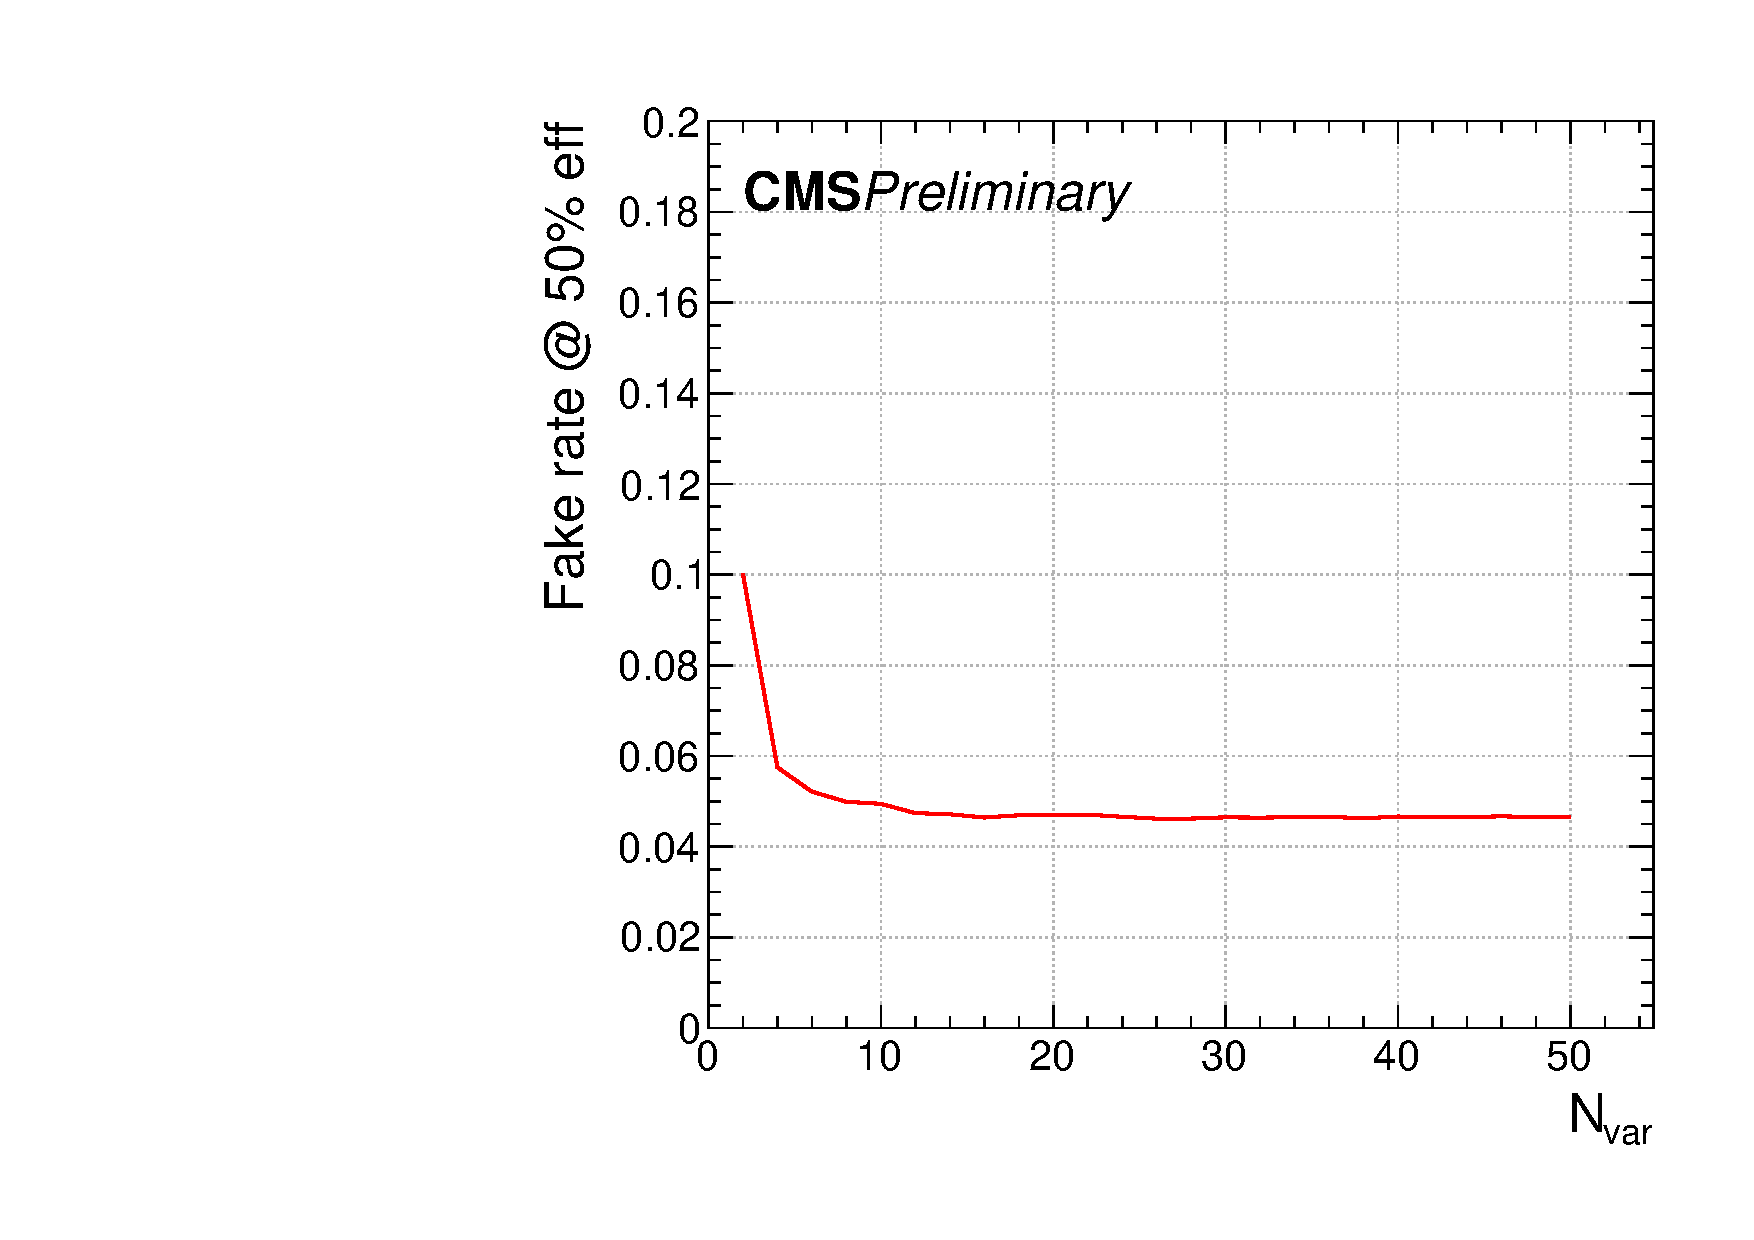
\includegraphics[width=\textwidth]{figures/toptagging/bdt/fakerate_vs_eff50.pdf}
        \end{subfigure}
        \caption{Performance of BDTs as a function of the number of ECF ratios used in the training.}
        \label{fig:jets:training}
    \end{center}
\end{figure}

\section{Data validation}
\label{sec:jets:sf}
